%Version 3 October 2023
% See section 11 of the User Manual for version history
%
%%%%%%%%%%%%%%%%%%%%%%%%%%%%%%%%%%%%%%%%%%%%%%%%%%%%%%%%%%%%%%%%%%%%%%
%%                                                                 %%
%% Please do not use \input{...} to include other tex files.       %%
%% Submit your LaTeX manuscript as one .tex document.              %%
%%                                                                 %%
%% All additional figures and files should be attached             %%
%% separately and not embedded in the \TeX\ document itself.       %%
%%                                                                 %%
%%%%%%%%%%%%%%%%%%%%%%%%%%%%%%%%%%%%%%%%%%%%%%%%%%%%%%%%%%%%%%%%%%%%%

%%\documentclass[referee,sn-basic]{sn-jnl}% referee option is meant for double line spacing

%%=======================================================%%
%% to print line numbers in the margin use lineno option %%
%%=======================================================%%

%%\documentclass[lineno,sn-basic]{sn-jnl}% Basic Springer Nature Reference Style/Chemistry Reference Style

%%======================================================%%
%% to compile with pdflatex/xelatex use pdflatex option %%
%%======================================================%%

%%\documentclass[pdflatex,sn-basic]{sn-jnl}% Basic Springer Nature Reference Style/Chemistry Reference Style


%%Note: the following reference styles support Namedate and Numbered referencing. By default the style follows the most common style. To switch between the options you can add or remove “Numbered” in the optional parenthesis. 
%%The option is available for: sn-basic.bst, sn-vancouver.bst, sn-chicago.bst%  
 
%%\documentclass[sn-nature]{sn-jnl}% Style for submissions to Nature Portfolio journals
%%\documentclass[sn-basic]{sn-jnl}% Basic Springer Nature Reference Style/Chemistry Reference Style
\documentclass[pdflatex,sn-mathphys-num]{sn-jnl}% Math and Physical Sciences Numbered Reference Style 
%%\documentclass[sn-mathphys-ay]{sn-jnl}% Math and Physical Sciences Author Year Reference Style
%%\documentclass[sn-aps]{sn-jnl}% American Physical Society (APS) Reference Style
%%\documentclass[sn-vancouver,Numbered]{sn-jnl}% Vancouver Reference Style
%%\documentclass[sn-apa]{sn-jnl}% APA Reference Style 
%%\documentclass[sn-chicago]{sn-jnl}% Chicago-based Humanities Reference Style

%%%% Standard Packages
%%<additional latex packages if required can be included here>

\usepackage{graphicx}%
\usepackage{multirow}%
\usepackage{amsmath,amssymb,amsfonts}%
\usepackage{amsthm}%
\usepackage{mathrsfs}%
\usepackage[title]{appendix}%
\usepackage{xcolor}%
\usepackage{textcomp}%
\usepackage{manyfoot}%
\usepackage{booktabs}%
\usepackage{algorithm}%
\usepackage{algorithmicx}%
\usepackage{algpseudocode}%
\usepackage{listings}%
\usepackage{bm}
\usepackage{macros}

%%%%

%%%%%=============================================================================%%%%
%%%%  Remarks: This template is provided to aid authors with the preparation
%%%%  of original research articles intended for submission to journals published 
%%%%  by Springer Nature. The guidance has been prepared in partnership with 
%%%%  production teams to conform to Springer Nature technical requirements. 
%%%%  Editorial and presentation requirements differ among journal portfolios and 
%%%%  research disciplines. You may find sections in this template are irrelevant 
%%%%  to your work and are empowered to omit any such section if allowed by the 
%%%%  journal you intend to submit to. The submission guidelines and policies 
%%%%  of the journal take precedence. A detailed User Manual is available in the 
%%%%  template package for technical guidance.
%%%%%=============================================================================%%%%

%% as per the requirement new theorem styles can be included as shown below
\theoremstyle{thmstyleone}%
\newtheorem{theorem}{Theorem}%  meant for continuous numbers
%%\newtheorem{theorem}{Theorem}[section]% meant for sectionwise numbers
%% optional argument [theorem] produces theorem numbering sequence instead of independent numbers for Proposition
\newtheorem{proposition}[theorem]{Proposition}% 
%%\newtheorem{proposition}{Proposition}% to get separate numbers for theorem and proposition etc.

\theoremstyle{thmstyletwo}%
\newtheorem{example}{Example}%
\newtheorem{remark}{Remark}%

\theoremstyle{thmstylethree}%
\newtheorem{definition}{Definition}%

\raggedbottom
%%\unnumbered% uncomment this for unnumbered level heads

\begin{document}

\title{Decoding Fossil Floras with Artificial Intelligence: An application to the Florissant formation}
% \title{Identifying fossil leaves to family using deep neural networks: example from the Florissant flora}
\author*[1,2]{\fnm{First} \sur{Author}}\email{iauthor@gmail.com}

\author[2,3]{\fnm{Second} \sur{Author}}\email{iiauthor@gmail.com}
\equalcont{These authors contributed equally to this work.}

\author[1,2]{\fnm{Third} \sur{Author}}\email{iiiauthor@gmail.com}
\equalcont{These authors contributed equally to this work.}

\affil*[1]{\orgdiv{Department}, \orgname{Organization}, \orgaddress{\street{Street}, \city{City}, \postcode{100190}, \state{State}, \country{Country}}}

\affil[2]{\orgdiv{Department}, \orgname{Organization}, \orgaddress{\street{Street}, \city{City}, \postcode{10587}, \state{State}, \country{Country}}}

\affil[3]{\orgdiv{Department}, \orgname{Organization}, \orgaddress{\street{Street}, \city{City}, \postcode{610101}, \state{State}, \country{Country}}}

%% Suggested author list: Rodriguez* Fel* Gonkar Vaishnav Meyer Wilf** Serre**
% Just a proposal. Let me (TS) know if you disagree. Also anybody that I forgot?

\abstract{
Accurately identifying fossil angiosperm leaves remains a longstanding challenge in paleobotany. While the morphological complexity of leaves has historically hindered manual classification, artificial intelligence (AI) appears well-suited to extract subtle diagnostic patterns that may elude human perception. However, applying standard AI approaches to fossil material faces a fundamental limitation: the extreme scarcity of taxonomically vetted fossil specimens precludes conventional supervised training at scale.

Here we introduce a deep learning framework that overcomes this challenge by augmenting sparse fossil data with synthetic examples and aligning extant and fossil domains through representational learning. Our approach synthesizes high-fidelity fossil analogs from modern leaf images (cleared and X-rayed) and trains a deep neural network using multi-scale representations with triplet-loss embedding to align fossil and extant domains. The resulting system achieves 91.8\% top-5 accuracy (chance: 3.5\%) for family-level classification of fossil leaves and, remarkably, 73.4\% accuracy even for fossil families excluded from training—demonstrating robust out-of-distribution generalization. To reveal the model's decision process, we developed a concept-based interpretability framework that extracts and localizes visual features driving classification decisions. We demonstrate practical utility by applying our system to 1,723 previously unidentified fossils from the Florissant Formation, providing predictions with visual explanations to guide expert review. By overcoming data scarcity through generative AI and representational learning, this work offers a pathway to unlock large-scale paleobotanical ``dark data."
}
\maketitle



Isolated leaves dominate the angiosperm fossil record yet remain notoriously difficult to identify accurately, representing paleobotany's largely untapped "dark data"—vast collections of specimens that remain scientifically inaccessible due to taxonomic ambiguities. Historical literature contains numerous uncertain or incorrect botanical identifications, largely due to morphological similarities between families, substantial variation across fossil sites, uneven preservation conditions, and a scarcity of reliably identified reference specimens. Accurate fossil leaf classification is crucial, however, as leaves provide essential data for reconstructing past biodiversity, climate conditions, and ecosystem composition.

Artificial intelligence (AI), particularly deep learning, has shown promise in botanical research for automated plant species classification~\cite{plantclassificationGunjal2024,machinelearningspecies}. Yet AI-based approaches face similar limitations to human experts when applied to fossils: limited samples and substantial site-to-site variability. Pronounced taphonomic variation across different sites significantly hampers model generalization, as confirmed by our initial exploratory analyses. To systematically evaluate and optimize deep learning methods under controlled conditions, we therefore restricted this study to a single, exceptionally well-documented fossil site.

We focused on the late Eocene Florissant Fossil Beds National Monument in Colorado, where taphonomic conditions are comparatively consistent and thoroughly documented. The Florissant flora was systematically described in MacGinitie's seminal 1953 monograph~\cite{mcginitie1953fossil} and subsequently expanded by Manchester and colleagues. Meyer's digital archive~\cite{florissant} comprises thousands of specimens and represents one of the earliest large-scale paleobotanical image datasets available online. From this resource, we extracted 3,200 vetted fossil leaves covering 23 plant families, including 16 families with at least five specimens each. These vetted fossils were selected from a larger Florissant dataset containing over 1,723 additional specimens that could not be confidently assigned to family level. Together, these images form part of an openly accessible compilation of fossil, cleared, and X-rayed leaves totaling 30,252 samples~\cite{wilf2021dataset}, recently augmented by 4,076 specimens from the National Museum of Nature and Science in Japan.

Most well-identified fossil leaves represent a handful of morphologically distinctive families that are well-represented in the literature, leaving the vast majority of angiosperm diversity in the fossil record unrecognized~\cite{Wilf2008FossilLeaves}. To address the fundamental limitation that fossil leaves frequently represent families with minimal or no direct fossil training samples, we employed generative AI to synthesize fossil-like images from a large dataset of cleared and X-rayed leaves spanning 142 modern families (each with at least 25 specimens) plus the 16 families of vetted fossils available. This approach greatly increases the number of angiosperm families available as "training fossils," substantially expanding the training data (Fig.~\ref{fig:system}). Adding synthetic fossil samples to the training dataset yielded considerable accuracy gains not only for families with real fossil examples available during training, but also for families represented only by synthetic fossils. This demonstrates the effectiveness of generative AI in overcoming inherent data scarcity in paleobotany, enabling robust identification even when direct fossil representatives are lacking.
\begin{figure}[H]
    \centering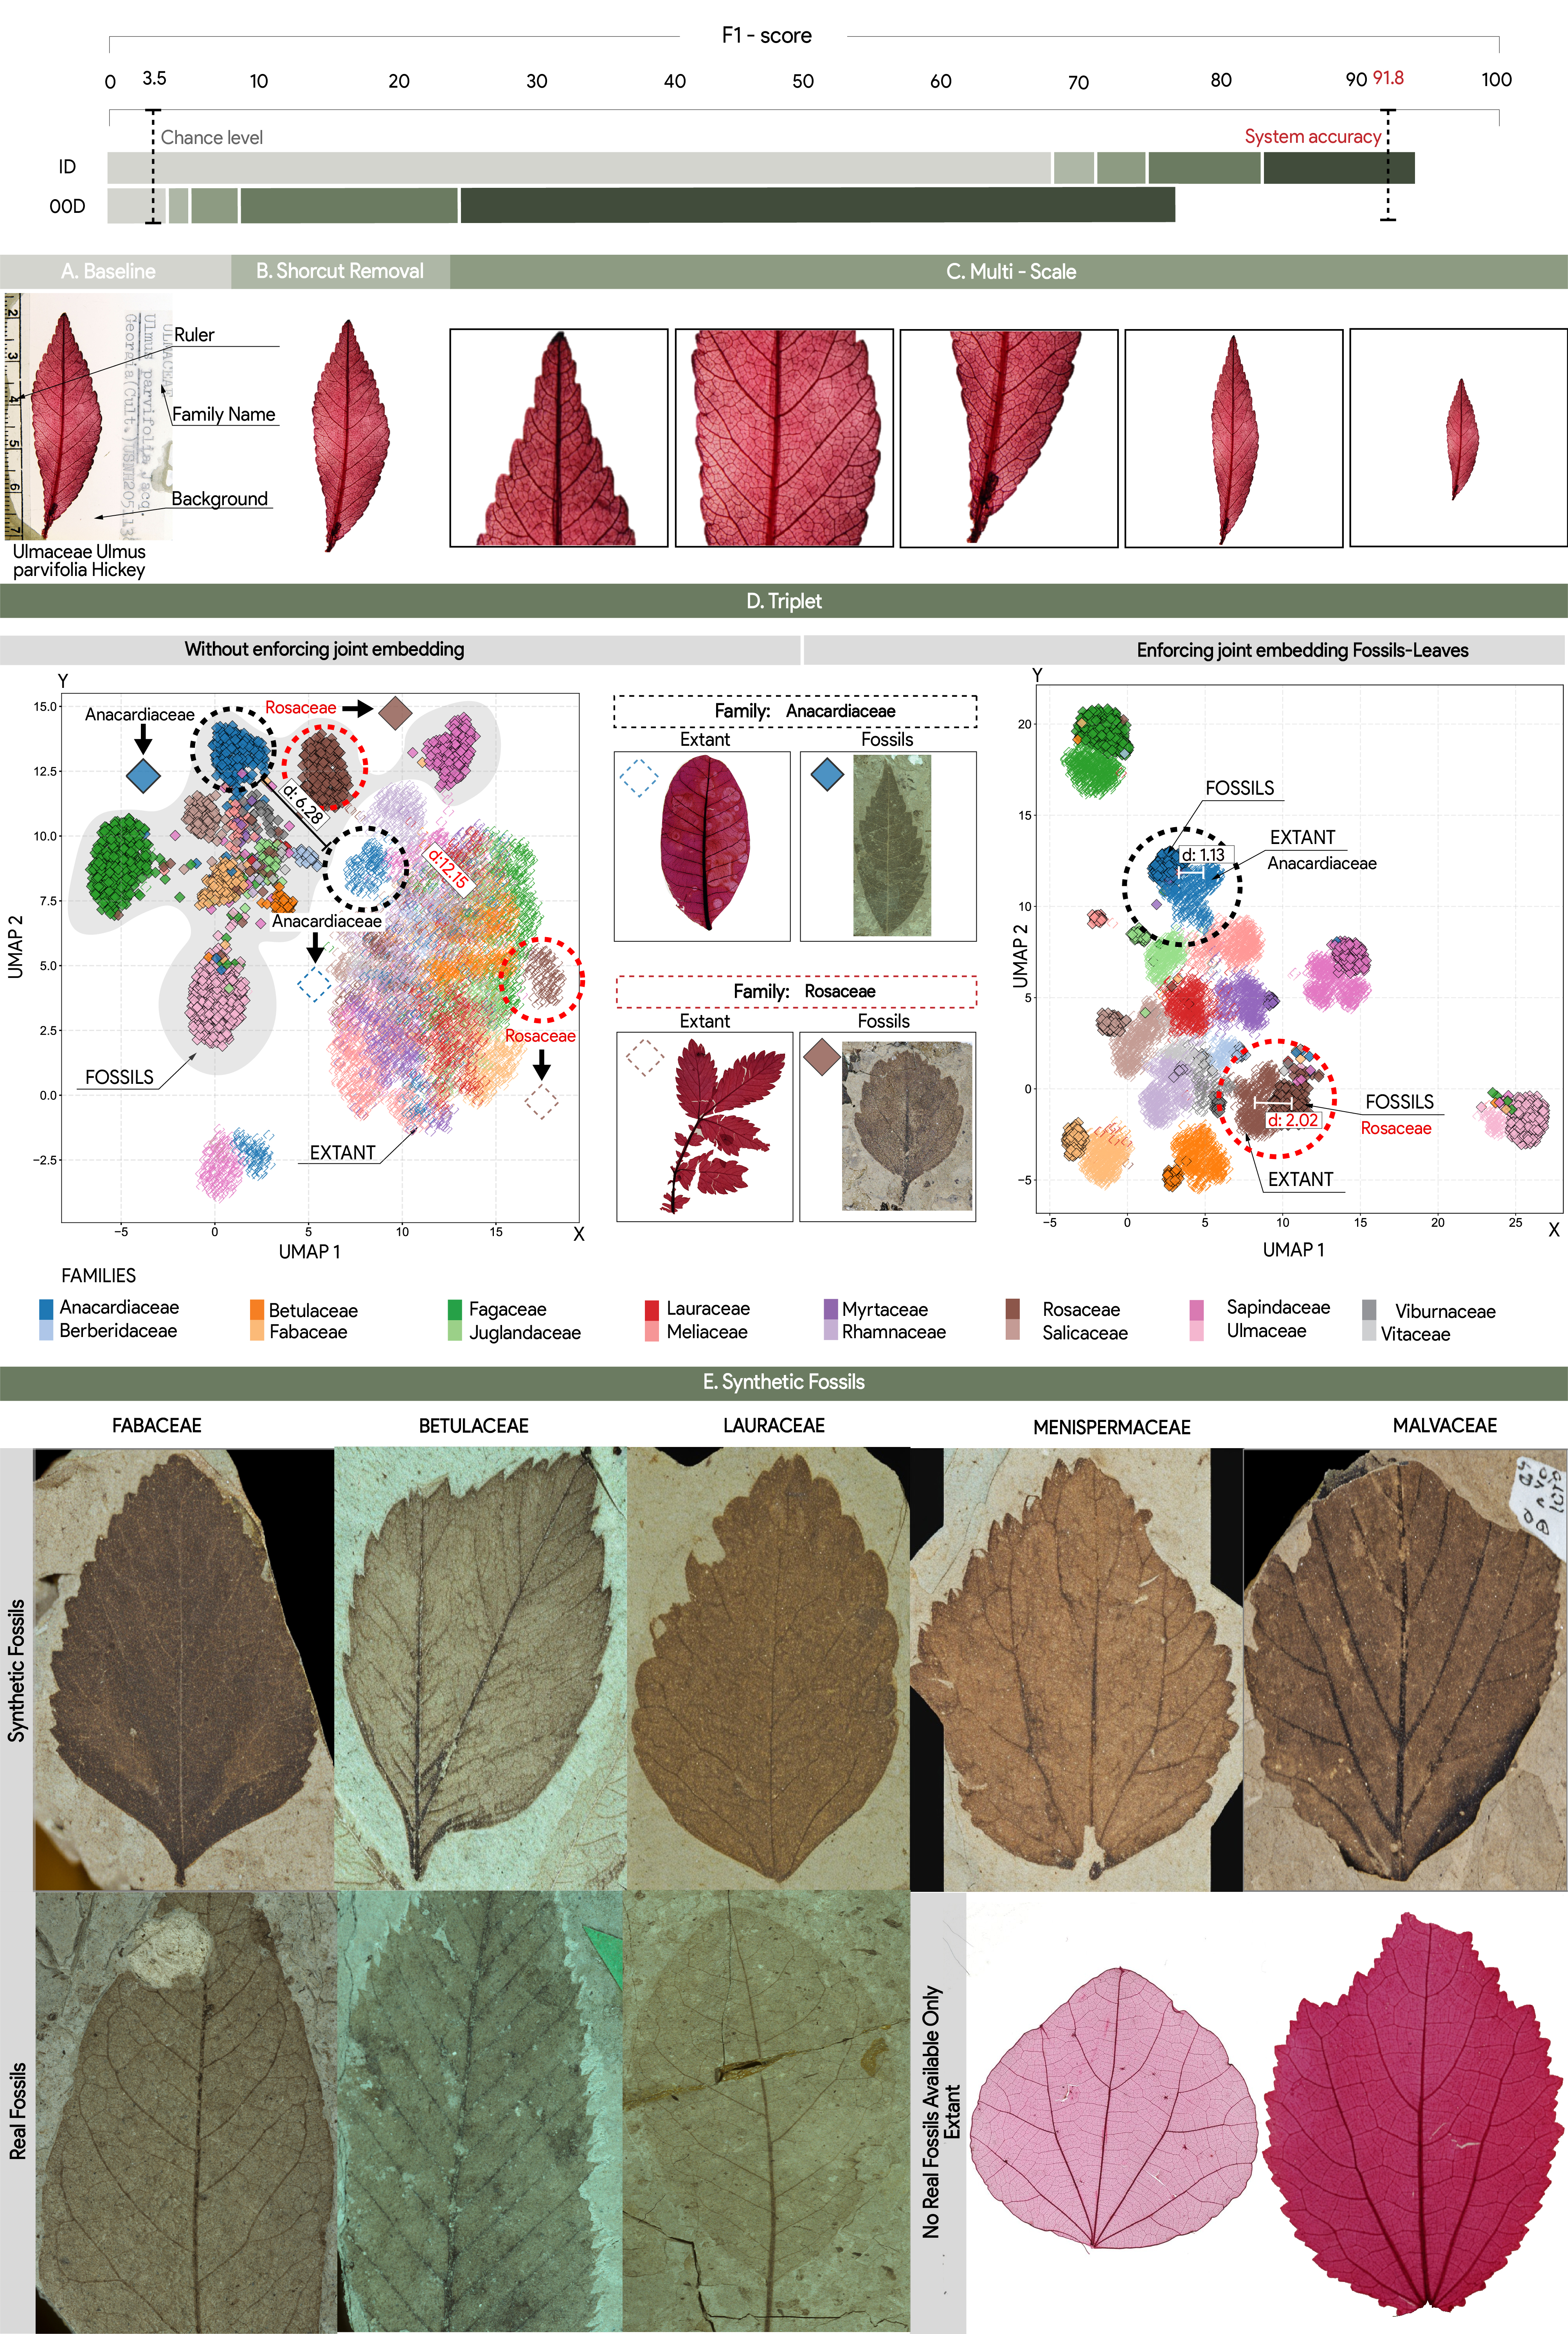
\includegraphics[width=\linewidth]{Figures/Figure_1_v6.jpg}
    \caption{Model improvements for fossil leaf family identification and their cumulative effects on classification performance.
    \textbf{Performance bounds.} Bar chart shows Top-5 $F_1$ scores under two generalization scenarios: ``in-distribution (ID)'' uses real fossil leaves during training , while ``out-of-distribution (OOD)'' uses only synthetic fossils during training (simulated-to-real). Chance performance for 142 families is 3.5\% (dashed black  line). The final model achieves 91.8\% accuracy on combined extant and fossil leaves, with expected performance of 77.3\% (OOD) and 93.2\% (ID) on real fossils alone. \textbf{Model improvements (panels A–E):} (A) Raw extant leaf samples; (B) samples after automatic shortcut removal; (C) five-scale image pyramid enabling multi-resolution classification; (D) Using our triplet loss to enforce joint representation for both domains: On the left, visualization of clusters using UMAP showing that distance between samples of the same family are farther away than samples of the same domain. On the right, the impact of our loss, bringing samples of the same family closer on the feature space regardless of the domain ; (5) high-fidelity synthetic fossils generated to augment under-represented families and those lacking fossil specimens. On top examples of our generated synthetic fossils, on the bottom samples of existing fossils from a sample of the same family and two original extant leaves that serve as a source when real family not available.}
    \label{fig:system}
\end{figure}
\section*{Results}

We developed our deep learning architecture through multiple iterations and cumulative improvements built upon a ResNet-101 backbone~\cite{resnetHe2015}, a widely-used 101-layer convolutional neural network with strong performance in computer vision tasks (Fig.~\ref{fig:system}). Throughout this work, we report top-5 accuracy—the proportion of test images for which the correct family label appears among the five highest-ranked predictions. Chance-level performance for this 142-family classification task is 3.5\%. We conducted all experiments using 80\%/10\%/10\% training/validation/test splits, with comprehensive grid search optimization of hyperparameters based on validation performance. All accuracy measures reflect test-set results averaged across $n = 10$ independent stratified random splits.


Our trained ResNet-101 model achieved 91.8\% overall test accuracy across extant and fossil leaves. However, evaluating fossil-specific performance presents a key challenge: our dataset contains vetted fossil specimens for only 16 of the 142 families. To quantify classification accuracy specifically for fossil leaves, we restricted our test set to these 16 families while maintaining classification across all 142 families. 

We evaluated two scenarios to establish performance bounds. In the \textbf{in-distribution (ID)} scenario, real fossil specimens from the test family were included during training, with evaluation performed on unseen real specimens of the same family using standard train/validation/test splits. This yielded an average accuracy of 67.3\%. In the more challenging \textbf{out-of-distribution (OOD)} scenario, we adopted a leave-one-family-out protocol where all real fossils from one family were withheld during training, and the model was tested on the complete set of real leaves from that excluded family. We repeated this process for each of the 16 families with 10 random initializations per model, resulting in $16 \times 10 = 160$ total runs. This OOD evaluation yielded an overall accuracy of 3.82\%, reflecting the considerably greater difficulty of bridging the simulation-to-reality gap when synthetic data must substitute for real specimens (Fig.~\ref{fig:system}).
\begin{figure}[ht!]
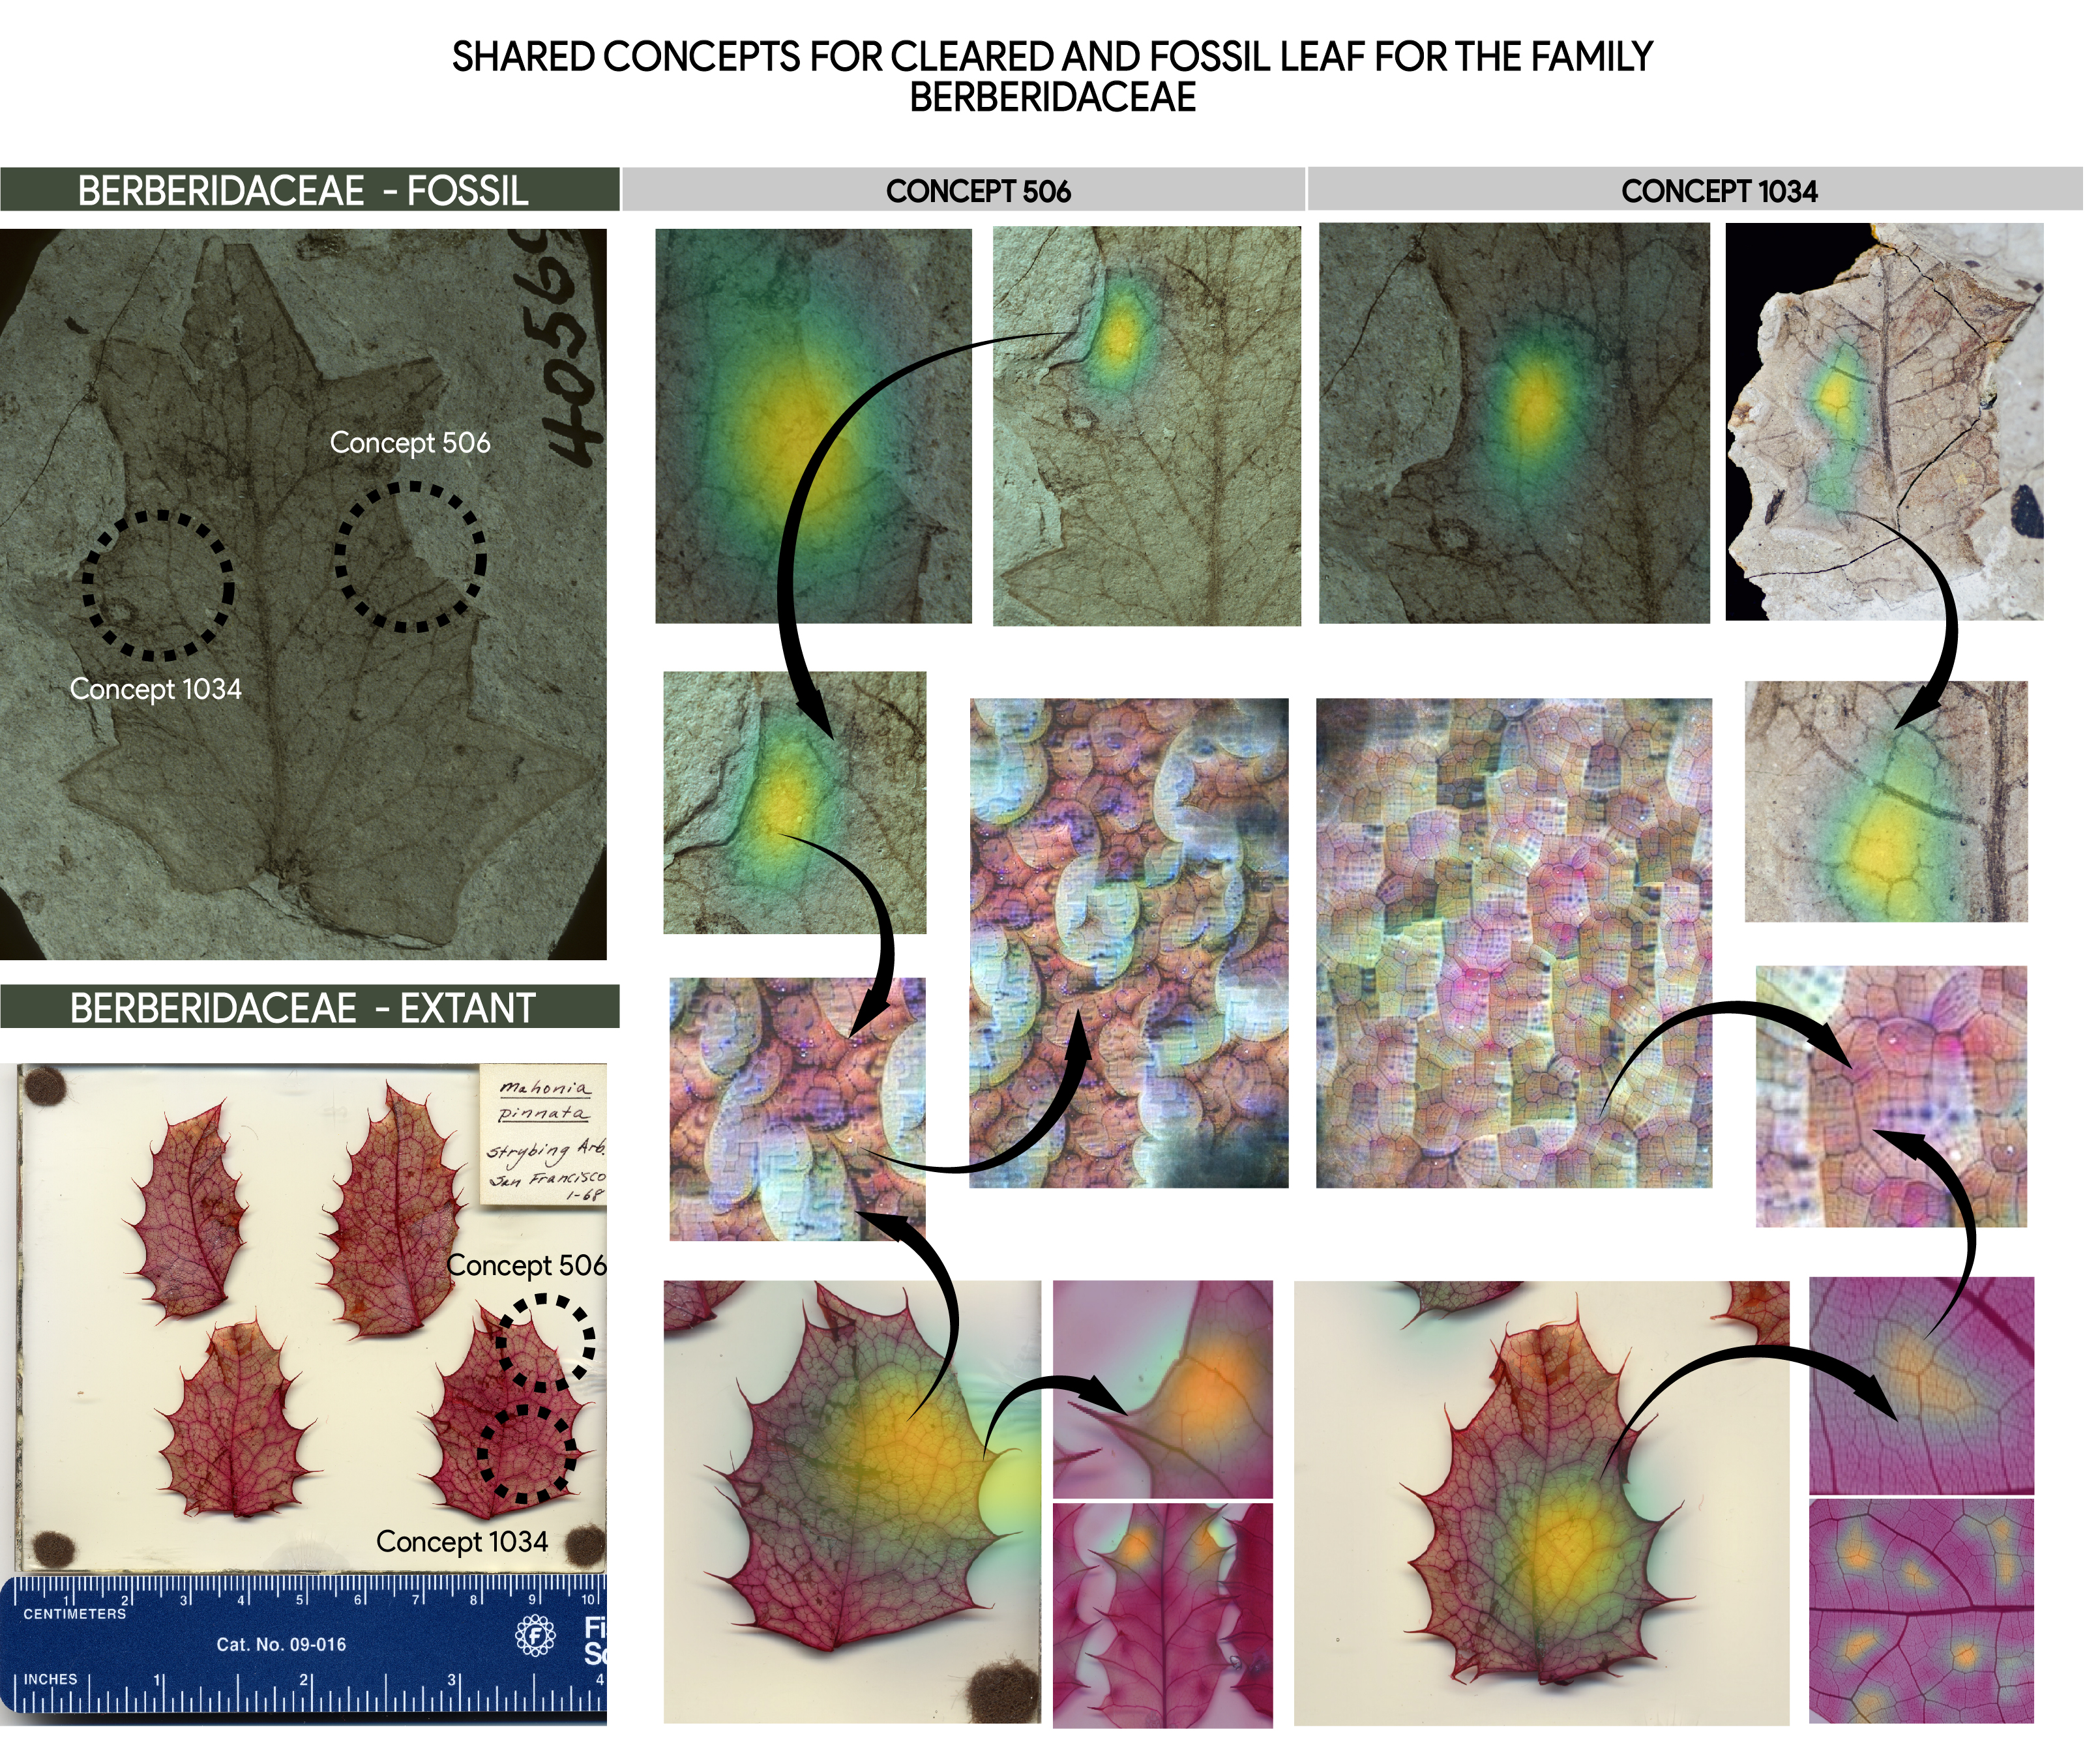
\includegraphics[width=\linewidth]{Figures/Figure_3_v3.jpg}
    \caption{Shared concepts used by the model to classify an example from the class  Berberidaceae. }
    \label{fig:shared_concepts}
\end{figure}
A common challenge in deep learning is the tendency for neural networks to rely on spurious correlations—so-called shortcuts—between image backgrounds or annotations and class labels. This issue is particularly problematic in scientific applications, where hidden data acquisition biases, annotation artifacts, or preparation procedures can lead models to overfit to unintended cues rather than meaningful biological features~\citep{Brown2023ShortcutTesting,Nauta2022SkinShortcut,Hill2024ShortcutRisk}. 
\begin{figure}
    \centering
    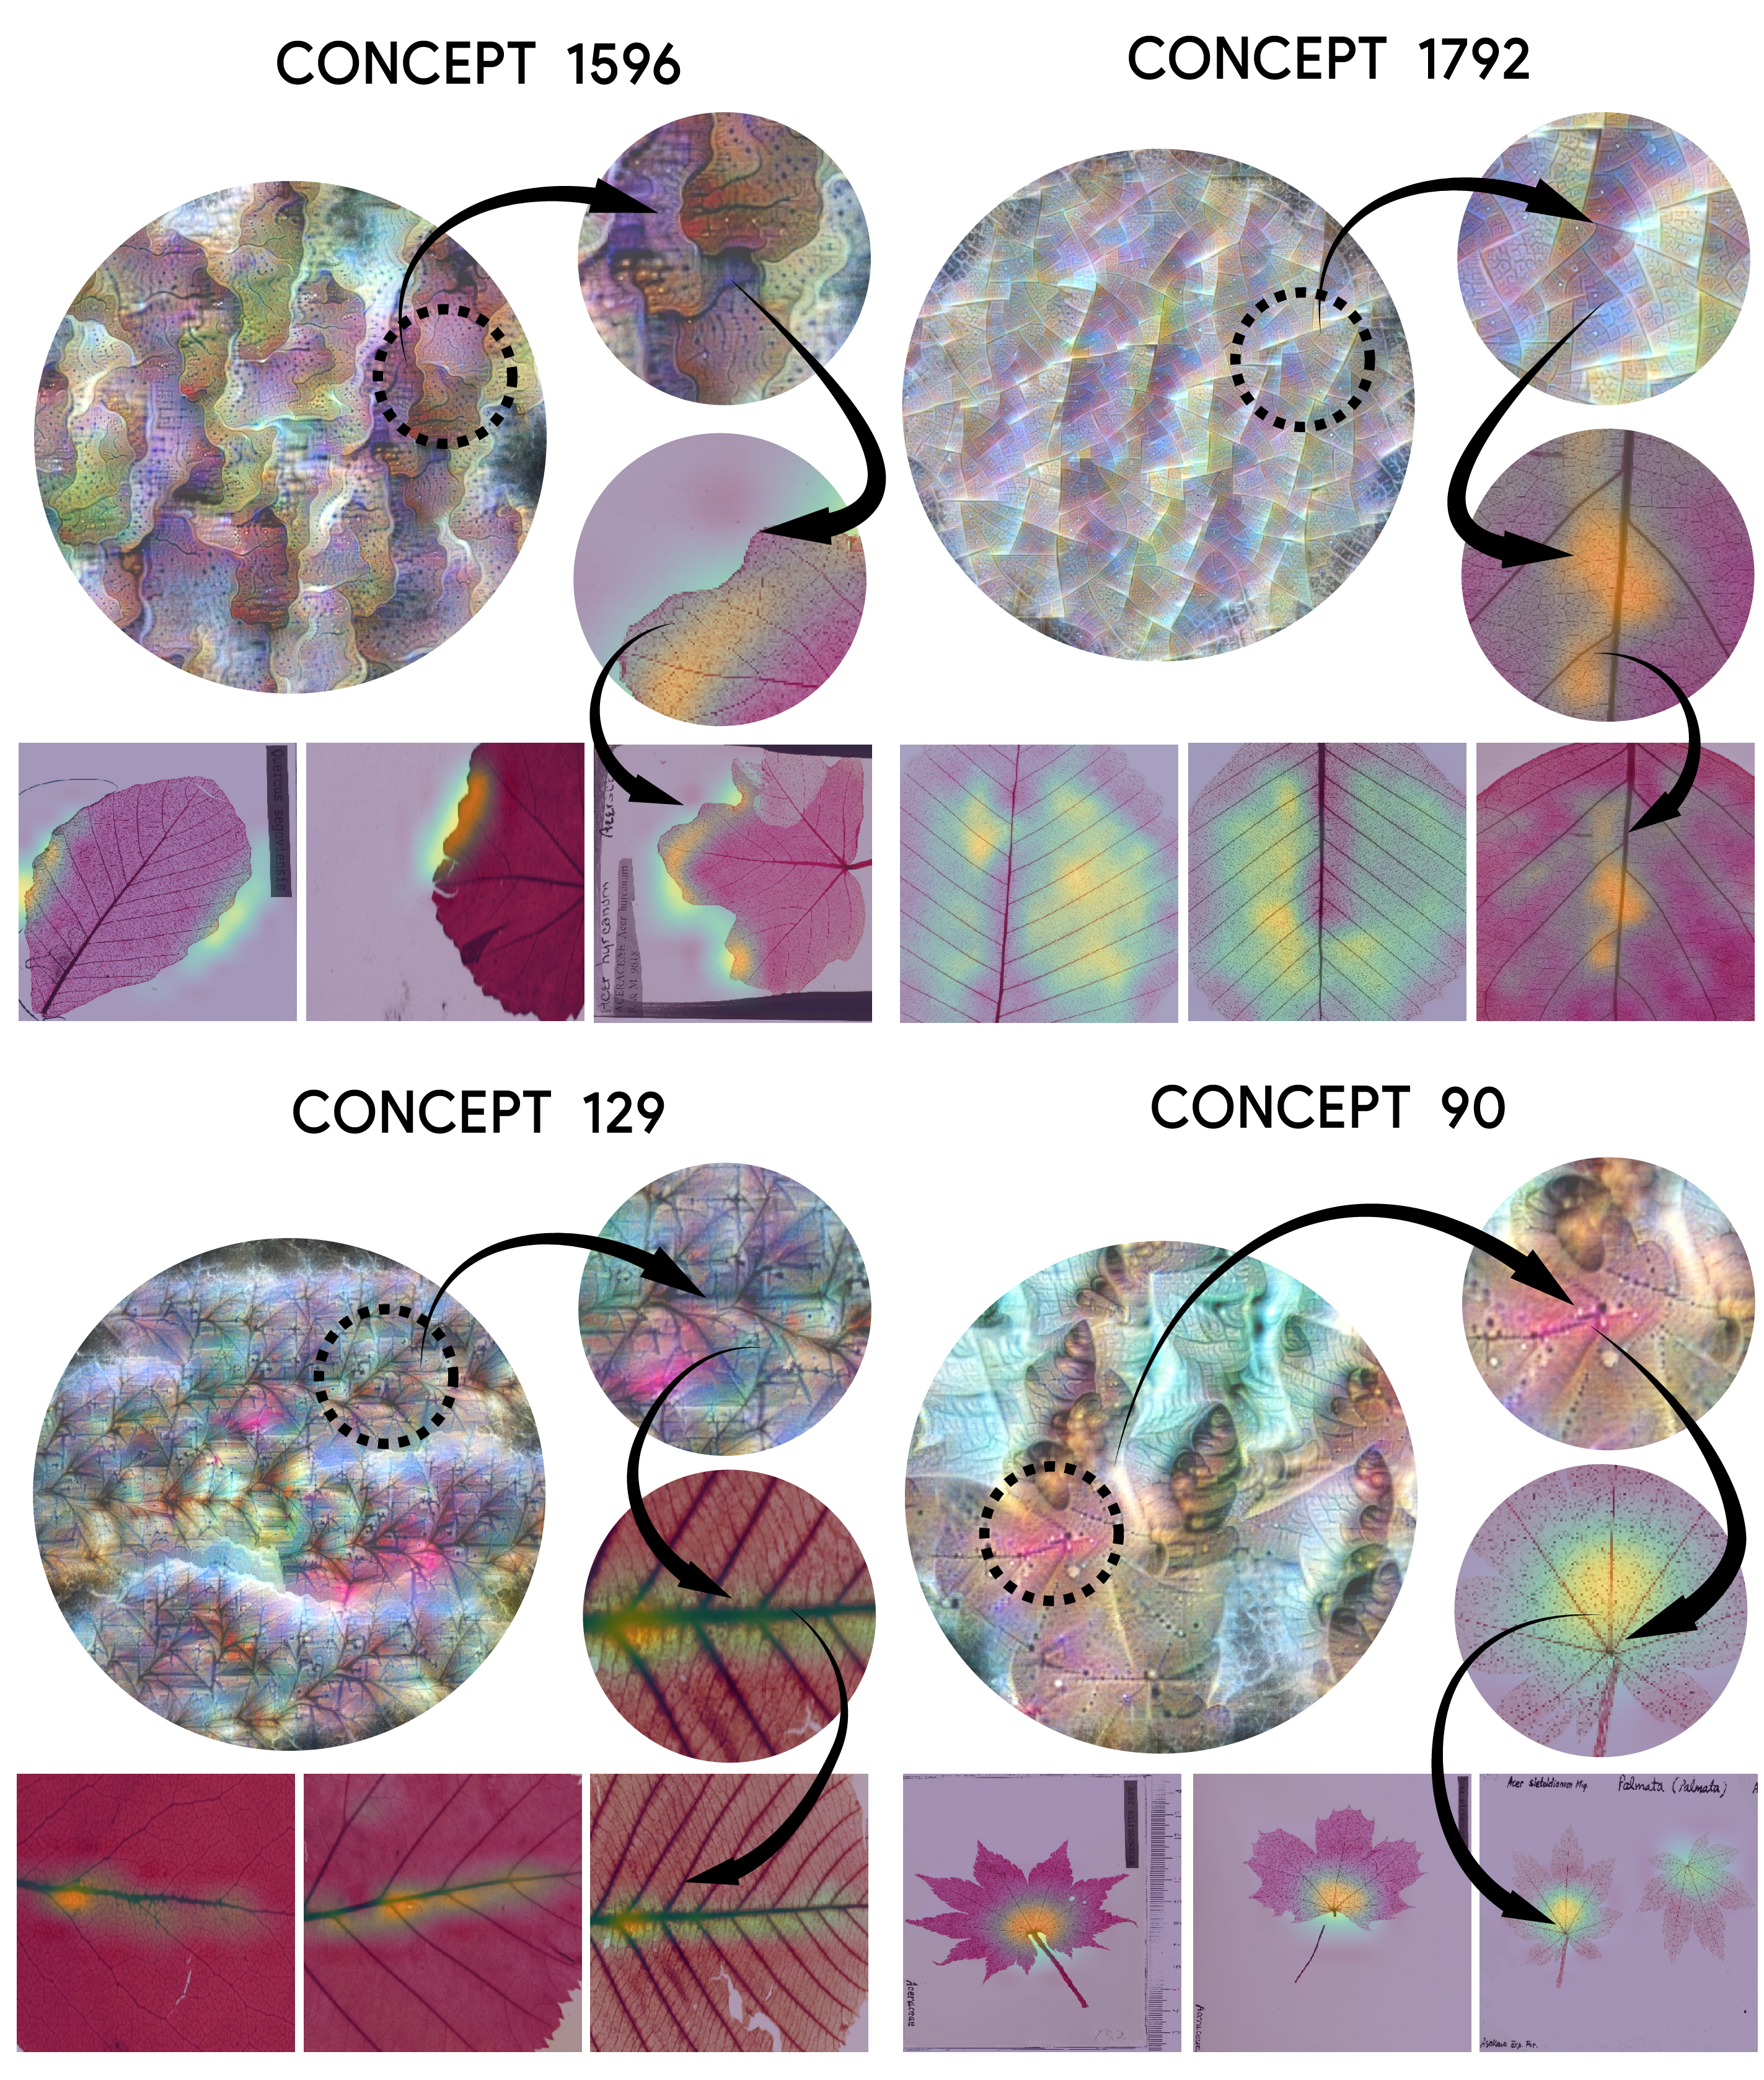
\includegraphics[width=\linewidth]{Figures/Figure_6_v2.jpg}
    \caption{Examples of concepts used for the model for classification. Concept 1596: Pattern in the border. Concept 1792: Secondary veins juctions with primary vein. Concept 129: Paternary Vein. Concept 90: Bottom Junction. Concept 1596: Pattern in the border. Concept 1792: Secondary veins junctions with primary vain. Concept 129: Paternary Vein. Concept 90: Bottom Junction. For more concepts see Fig~\ref{fig:SI_concepts} and Fig~\ref{fig:SI_concepts2}. For the full list please visit the website \footnote{\url{https://fel-thomas.github.io/Leaf-Lens/}} .} 
    \label{fig:concepts}
\end{figure}
To assess the robustness of our model against such shortcuts, we computed attribution maps using saliency methods from our custom Xplique toolbox~\citep{fel2022xplique}. Visual inspection revealed that the model sometimes based classifications partly on background elements, potentially due to biases in how family labels were distributed across collections and variations in slide preparation. The model also leveraged annotations and text on slides as classification cues (see Fig.~\ref{fig:attribution_maps} for more de. While these shortcuts might improve ID model accuracy, they likely harm OOD generalization to novel collections and fossil specimens with different backgrounds.

To address this issue, we fine-tuned the Segment Anything Model (SAM)~\cite{kirillov2023segment} using 576 manually annotated, cleared leaf images, enabling effective leaf segmentation from backgrounds. After applying this model to mask backgrounds across the entire dataset (Fig.~\ref{fig:system}), we confirmed that classification accuracy remained high (90.5\% for the whole system). Crucially, attribution maps now indicate that the model predominantly relies on leaf morphology rather than background artifacts or annotations (Fig.~\ref{fig:attribution_maps}) which in fact show improvement in our ID (4.6\%) and OOD (70.1\%)  evaluations.


% A common challenge in deep learning is the tendency for neural networks to rely on spurious correlations—so-called shortcuts—between image backgrounds or annotations and class labels \citep{Geirhos2020Shortcuts,Hermann2024Foundations}. This issue is particularly problematic in scientific and biomedical applications, where hidden data acquisition biases, annotation artifacts, or preparation procedures can lead models to overfit to unintended cues rather than meaningful structure\citep{Brown2023ShortcutTesting,Lin2024ShortcutSegmentation,Nauta2022SkinShortcut,Hill2024ShortcutRisk}. To assess the robustness of our model against such shortcuts, we computed attribution maps (heatmaps highlighting pixels influential to network decisions) using the saliency method provided by our custom-built Xplique toolbox~\citep{fel2022xplique}. Visual inspection revealed instances where the model based its classification partly on background elements, potentially due to inherent biases in the distribution of family labels across collections and variations in slide preparation. Moreover, we observed that annotations and text on slides were also leveraged by the model. Although these shortcuts might improve accuracy on the training dataset, they are likely detrimental to generalization, especially for novel collections and fossil specimens with substantially different backgrounds.To mitigate this issue, we fine-tuned the ``Segment Anything Model'' (SAM)~\cite{kirillov2023segment} using a small set of $576$ manually annotated cleared leaf images, enabling effective segmentation of leaves from backgrounds. After applying this model across the entire dataset to mask backgrounds (Fig.~\ref{fig:system}b), we confirmed that model accuracy remained high (yellow in Fig.~\ref{fig:system}a). Crucially, attribution maps now indicate that the model predominantly relies on the leaf itself rather than background or annotations (Fig.~\ref{fig:attribution_maps}).


We hypothesized that leaves encode diagnostic features across multiple spatial scales—from macroscopic traits such as overall shape and margin to mesoscopic patterns like venation. To capture this morphological information, we extended our architecture to process images at multiple scales. Each input image was decomposed into five sub-images: the original masked image, a tighter crop defined by the smallest bounding box enclosing the leaf mask, and three additional crops corresponding to the top, middle, and bottom thirds of the leaf (Fig.~\ref{fig:system}). This multiscale approach improved classification accuracy to 75.1\% and 8.72\% for ID and OOD accuracy, respectively.



% Our dataset exhibits a significant imbalance, comprising 34,328 extant and 3,200 fossil leaves—a ratio of approximately \(10{:}1\). Moreover, fossil leaves often differ markedly from extant specimens due to factors such as damage, partial preservation, compression artifacts, and the presence of rock matrix, which can obscure fine venation patterns. We hypothesized that these differences might lead the model to treat extant and fossil leaves as distinct domains. To investigate this, we computed the average within-family distances for extant and fossil leaves separately, normalizing each by the corresponding between-family average for that family. On average, fossil leaves were positioned farther from their extant counterparts than extant leaves from other families. This pattern is evident in Fig.~\ref{fig:system} , which presents a UMAP visualization of the neural network's penultimate layer embeddings, highlighting the domain shift between extant and fossil specimens.

% To address this domain shift, we turned to representation learning and introduced a \textbf{triplet-loss} regularizer to the classification objective during model training (\textit{Methods}). This regularizer explicitly encourages embedding representations that position fossil and extant leaves from the \emph{same} family closer together than fossil and extant leaves from \emph{different} families. Incorporating this constraint substantially improved model accuracy (82.3\%ID and 24.6\% OOD), with the greatest performance gains observed in the OOC condition, i.e., for families for which vetted fossil examples were unavailable during training.

% One remaining significant challenge is the complete absence of fossil specimens for most families in our dataset (119 of 142 families), with an additional seven families having fewer than five samples. To address this limitation, we leveraged generative AI by adapting a state-of-the-art stable diffusion model based on the ControlNet architecture~\citep{zhang2023adding}. Originally pre-trained on the LAION 5-billion image dataset, this conditional diffusion model synthesizes images guided by text prompts. We fine-tuned ControlNet to generate realistic images of cleared leaves and fossil specimens, training it jointly with our ResNet-101 family-level classifier. This joint training optimized a combined objective: classification accuracy for cleared and fossil leaves, a triplet-loss term to align extant and fossil representations within families, and the ControlNet loss itself. Representative synthetic fossil samples are shown in Figure~\ref{fig:system}. Crucially, this generative augmentation substantially improved the system's out-of-distribution generalization—classifying fossil leaves from families without real fossil examples available during training—raising accuracy dramatically from near-chance levels (3.82\%; Fig.~\ref{fig:system}, lower bound) to 77.3\% (upper bound), and narrowing the gap between in-distribution and out-of-distribution performance.

Our dataset exhibits significant imbalance, comprising 34,328 extant and 3,200 fossil leaves—approximately a 10:1 ratio. Moreover, fossil leaves often differ markedly from extant specimens due to damage, partial preservation, compression artifacts, and rock matrix that can obscure fine venation patterns. We hypothesized that these differences might lead the model to treat extant and fossil leaves as distinct domains.To investigate this, we measured the average distance in embedding space between fossil and extant samples within each family, and normalized this by the average distance between different families. After applying the triplet loss, these normalized distances decreased substantially, indicating that the model learns to cluster fossil and extant leaves from the same family together. A pattern evident in the UMAP visualization of the neural network's penultimate layer embeddings (Fig.~\ref{fig:sytem}).

To address this domain shift, we turned to representation learning and introduced a \textbf{triplet-loss} regularizer to the classification objective during model training (\textit{Methods}). This approach explicitly encourages embedding representations that position fossil and extant leaves from the same family closer together than those from different families. Incorporating this constraint substantially improved model accuracy to 82.3\% ID and 24.6\% OOD accuracy, with the greatest gains observed in the OOD condition where vetted fossil examples were unavailable during training.

A remaining challenge is the complete absence of fossil specimens for most families in our dataset (119 of 142 families), with seven additional families having fewer than five samples. To address this limitation, we leveraged generative AI by adapting a stable diffusion model based on the ControlNet architecture~\citep{zhang2023adding}. Originally pre-trained on the LAION 5-billion image dataset, this conditional diffusion model synthesizes images guided by text prompts. We fine-tuned the network to generate realistic cleared leaf and fossil images, training it jointly with our ResNet-101 classifier using a combined objective that includes classification accuracy, triplet-loss alignment of extant and fossil representations within families, and the ControlNet loss. This generative augmentation dramatically improved OOD generalization, raising OOD accuracy from near-chance levels (3.82\%) for our base model to 77.3\% , and from 6 93.2\% (ID) substantially narrowing the performance gap between the two evaluation reports. 


High-performing models often function as black boxes, making the rationale behind their predictions difficult to interpret. To address this, we developed an explainability framework~\cite{fel2024sparks} to identify internal visual concepts utilized by our fossil-leaf classification models, potentially uncovering diagnostic patterns difficult for human observers to discern~\cite{spagnuolo22}. Specifically, our interpretability framework comprises three key stages: (\textbf{\textit{i}}) concept extraction, (\textbf{\textit{ii}}) importance estimation, and (\textbf{\textit{iii}}) concept visualization.

% First, we \emph{extract} a structured and interpretable sparse dictionary of visual concepts from the model’s internal representations using a Top-\(k\) Sparse Autoencoder. This step is critical, as the internal feature space of deep neural networks often exhibits an overcomplete representation, with individual neurons encoding a superposition of multiple semantic factors. Direct analysis of raw activations could obscure this semantic structure, prompting us to employ sparse dictionary learning on intermediate-layer activations to derive a compact, disentangled set of visual primitives that the model relies upon~\cite{}.

% Second, we \emph{quantify} the importance of each extracted concept to the model’s predictions. Rather than assigning equal weight to all concepts, we reparameterize the classifier in concept space, directly attributing the model’s outputs to underlying concepts via a linear mapping. Each concept thus receives a class-specific importance score reflecting its influence on the decision boundary~\cite{}.

% Third, to make these concepts accessible and interpretable, we \emph{visualize} them spatially and semantically. Spatial visualization involves generating dense concept activation maps, clearly localizing concept activations within input images, while semantic visualization synthesizes prototypical input examples that selectively and maximally activate each concept~\cite{}. These three stages provide a structured, transparent decomposition of the model’s internal reasoning, enhancing human interpretability and trust in model predictions.


High-performing models often function as black boxes, making their decision-making rationale difficult to interpret. To address this, we developed an explainability framework to identify internal visual ``concepts'' utilized by our model, potentially uncovering diagnostic patterns difficult for human observers to discern~\cite{spagnuolo22}. Our interpretability framework comprises three key stages: \textbf{concept extraction}, \textbf{importance estimation}, and \textbf{concept visualization}.
\begin{figure}[H]
    \centering
    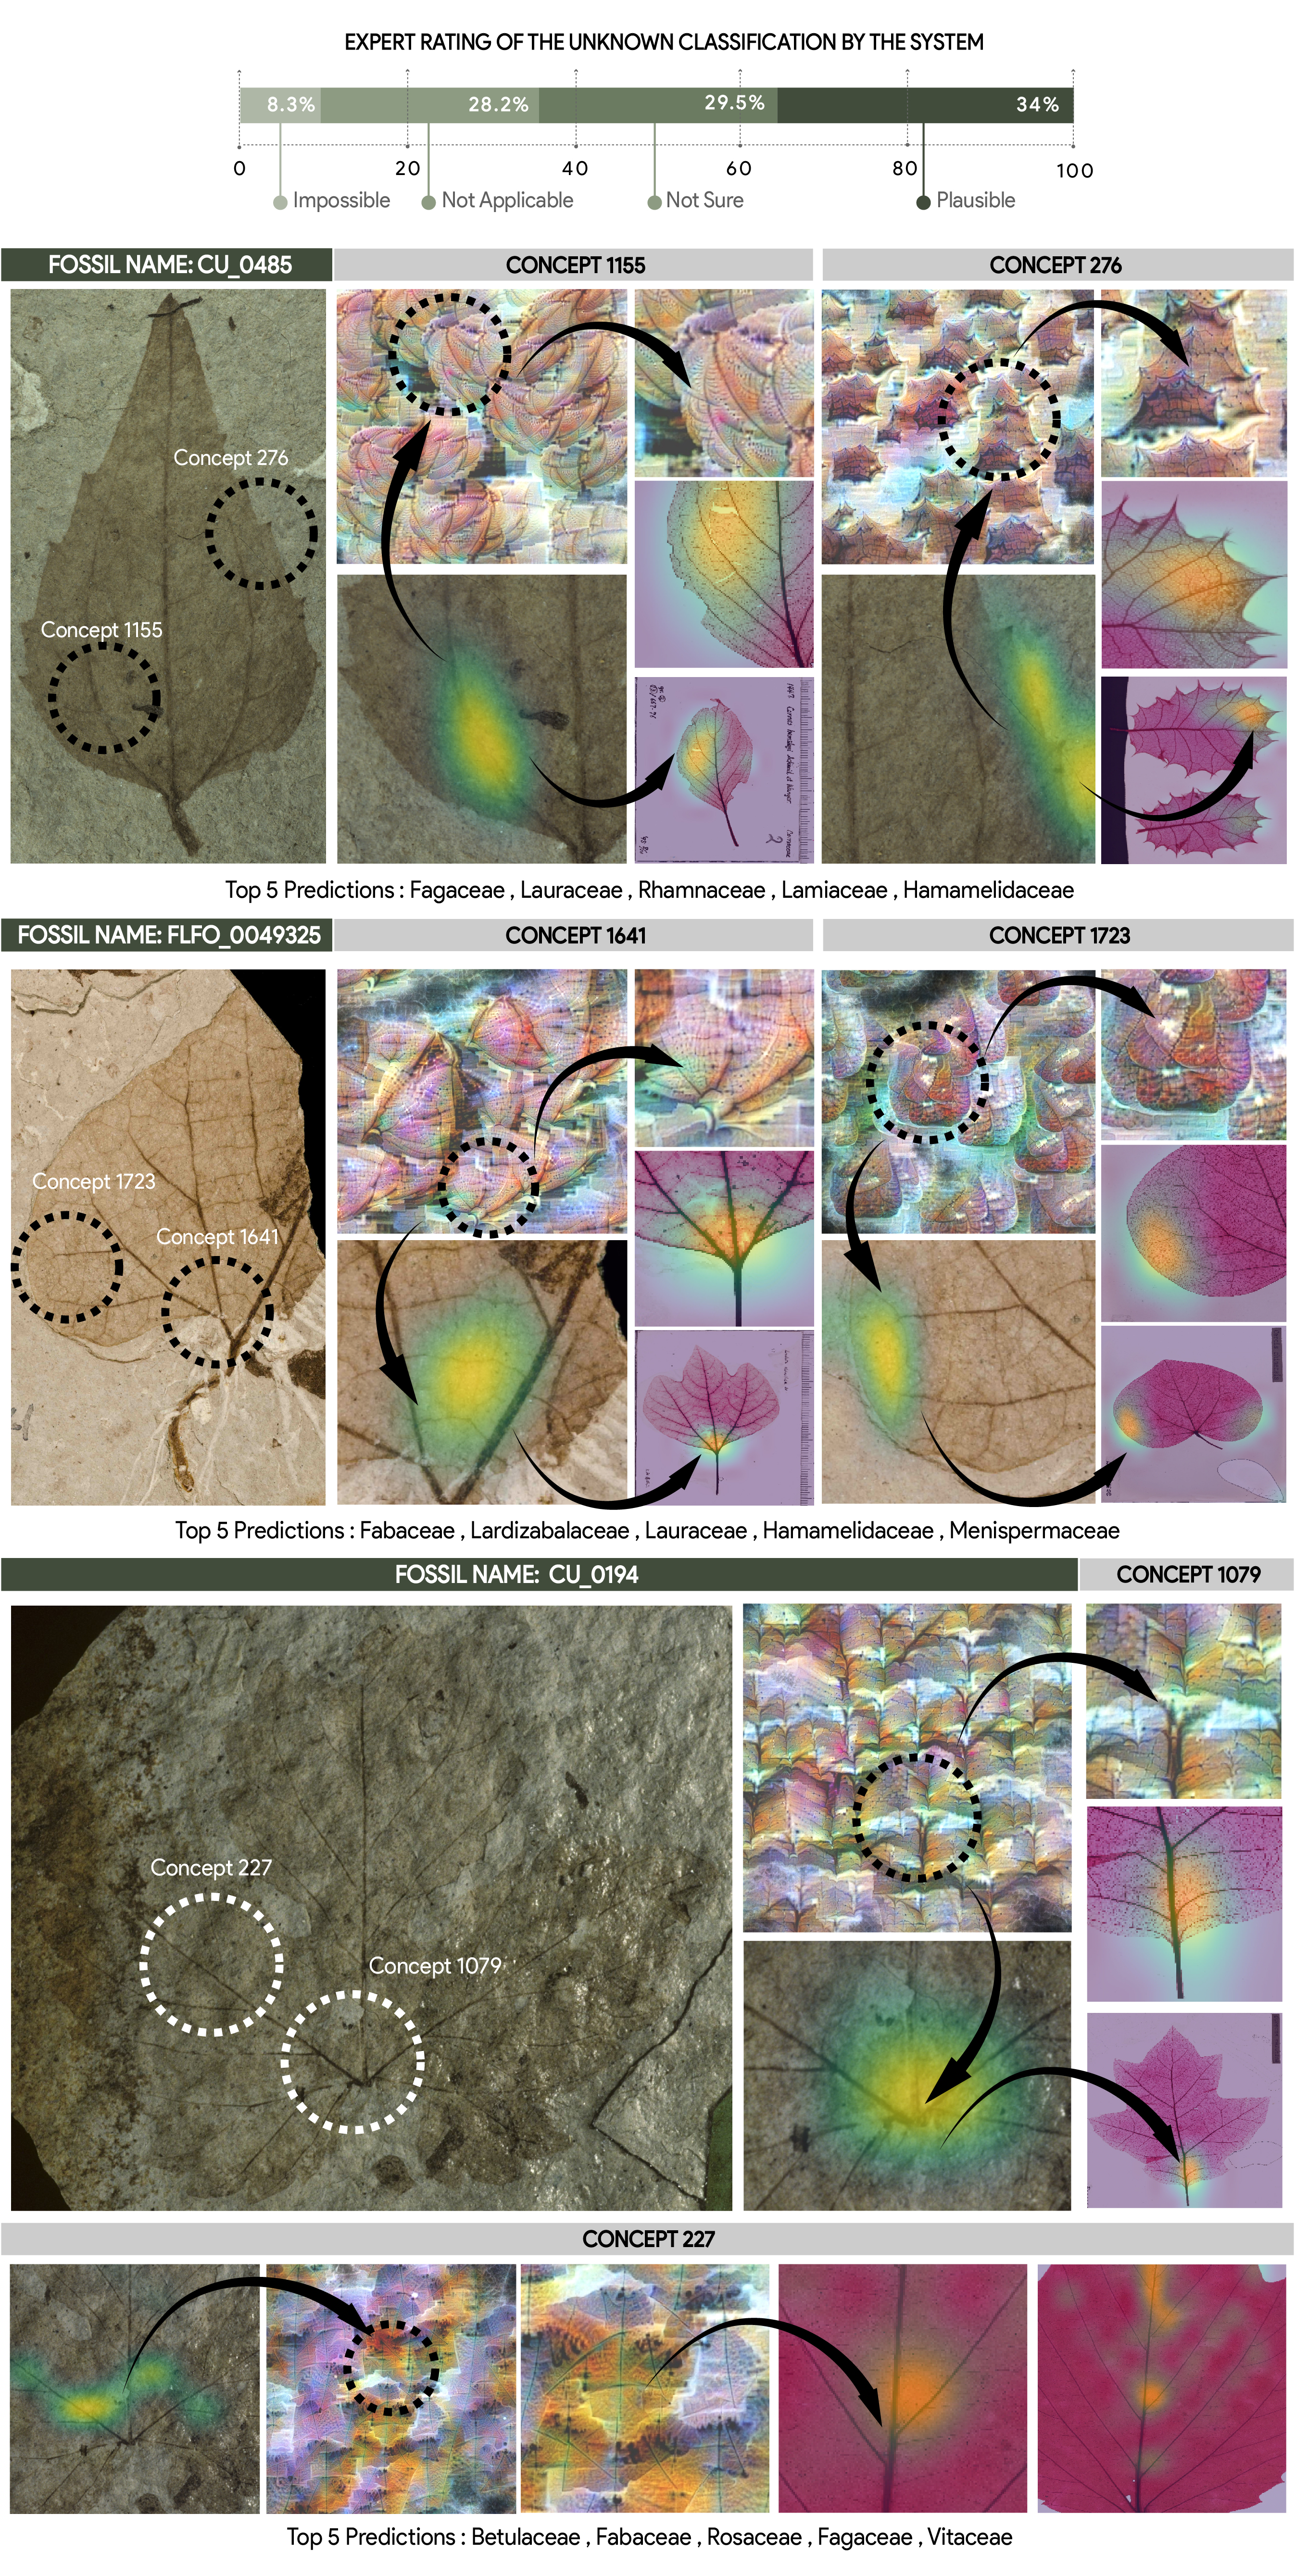
\includegraphics[width=0.9\linewidth]{Figures/Figure_2_v8.jpg}
    \caption{On top the distribution of the responses from the expert paleo-botanist evaluators. Examples of unidentified fossils their top 5 predictions from the model and the concepts used by the model to make such predictions. For instance, we find the arrangement of secondary veins, the pattern of dentation, the honey-comb pattern  and the junction between paternary and secondary veins.   }
    \label{fig:system2}
\end{figure}
First, we extract a structured dictionary of visual concepts from the model's internal representations using a Top-k Sparse Autoencoder~\cite{gao2024scaling}. This step is critical because deep neural networks often suffer from the problem of polysemanticity~\cite{elhage2022superposition}, with individual neurons encoding multiple semantic factors simultaneously. To avoid obscuring this semantic structure, we employ sparse dictionary learning~\cite{mairal2014sparse,olshausen1996emergence,tosic2011dictionary} on the penultimate layer activations~\cite{fel2023holistic} to derive a compact, disentangled set of visual concepts.

Second, we quantify the importance of each extracted concept for the model predictions. Rather than treating all concepts equally, we reparameterize~\cite{fel2023holistic}~the classifier in concept space, directly attributing model outputs to underlying concepts via linear mapping. Each concept receives a class-specific importance score reflecting its influence on the decision boundary.

Third, we visualize these concepts using Feature Visualization~\cite{olah2017feature,fel2023unlocking} in two ways to enhance interpretability: heat maps~\cite{zeiler2013visualizing,fong2017meaningful,petsiuk2018rise,fel2021sobol} indicate where individual concepts are activated within each image, and maximally exciting images reveal the visual patterns that most strongly activate each concept. Together, these stages provide a transparent decomposition of the model's internal reasoning, enhancing interpretability and trust in model predictions.


% \subsection{Explainability}






% To understand the decision-making process of our models, we employ explainability techniques such as Grad-CAM \cite{Selvaraju_2019} and RISE \cite{RISE2018} through the Xplique toolbox \cite{fel2022xplique}. These methods generate attribution maps highlighting the image regions that most influence predictions. 



% \begin{figure}[ht!]
%     \centering
%     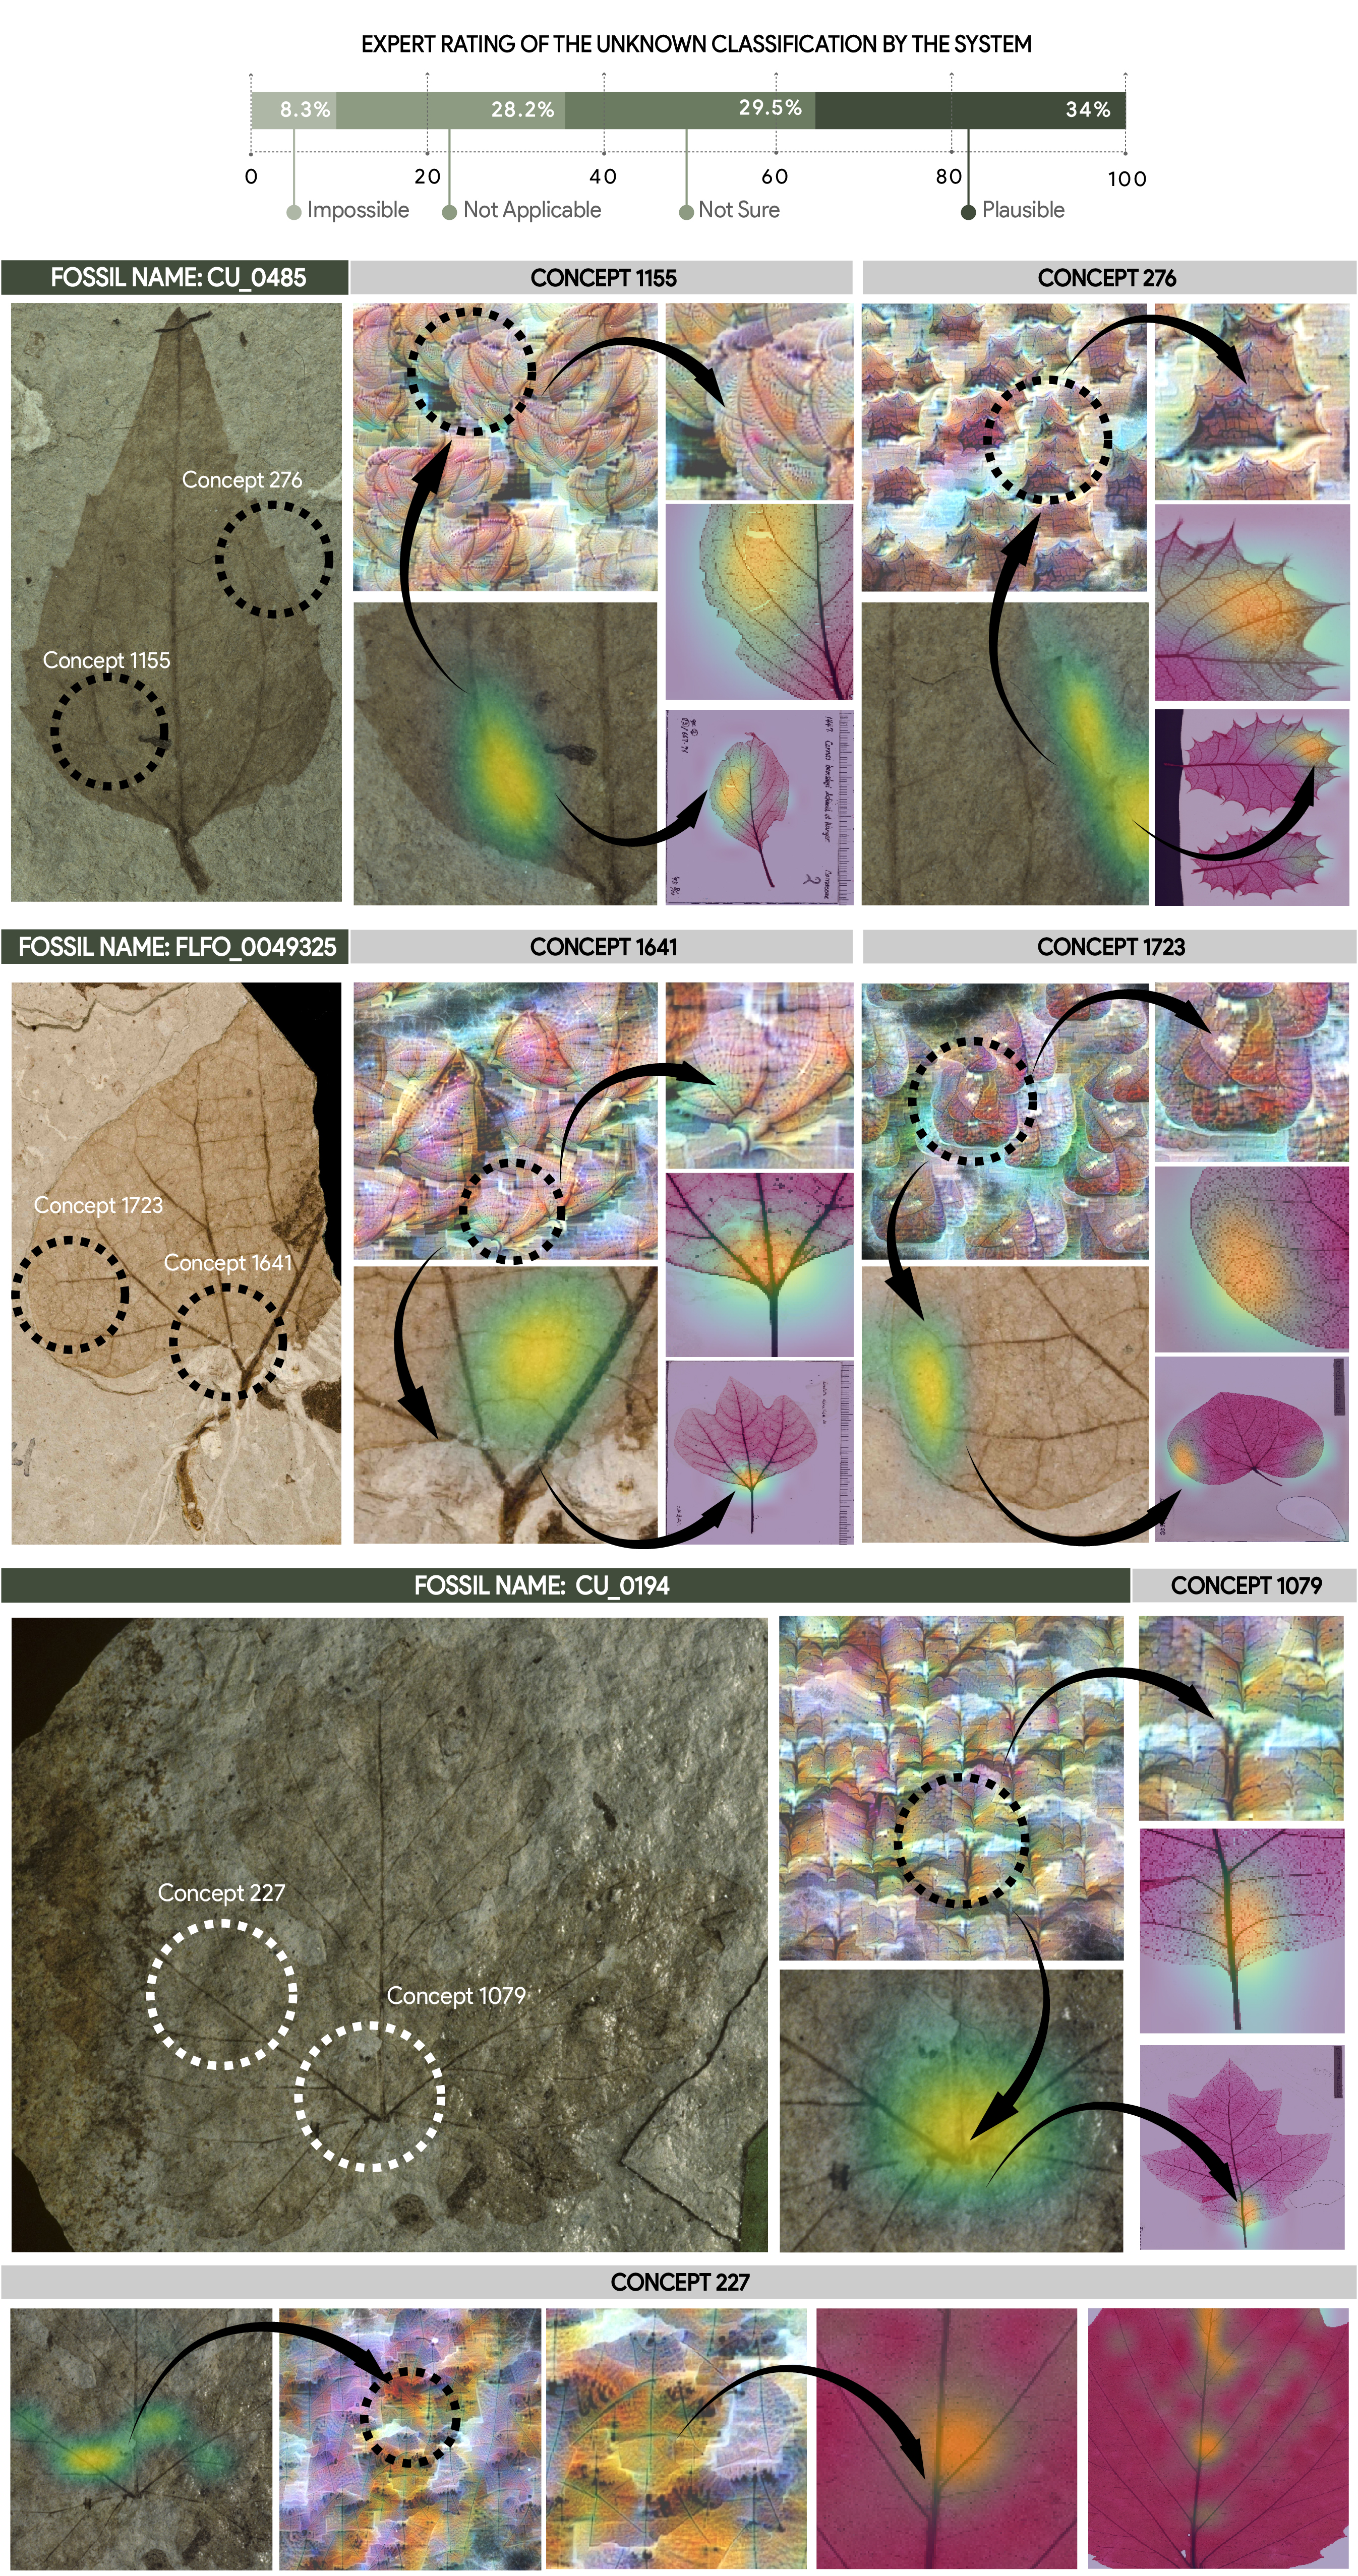
\includegraphics[width=\linewidth]{Figures/Figure_2_v7.jpg}
%     \caption{On top the distribution of the responses from the expert paleo-botanist evaluators. 8.3\% are predictions that are not possible, due to the fossil configuration. The  28.2\% of the fossils  were not applicable, meaning that their images were not properly taken and key features may have left out, or multiple leafs were present. 29.5\% are predictions that the expert are not sure and may constitute valuable cases were the concepts discovered by the system  can shed some light. 34\% of the cases were identified as plausible. The next row, there is an example of the Unidentified fossil, and the key concepts that were utilized for its classification, including the leaf formation on the left, the paternary vein in the middle and the junction between the paternary vein and the secondary veins.  }
%     \label{fig:system2}
% \end{figure}


Finally, we present the first machine-assisted classification of 1,723 fossil samples from the Florissant collection, encompassing specimens with previously unknown family labels or historical identifications no longer considered robust. The model's predictions and accompanying interpretability results were evaluated by two expert paleobotanists (P.W. and H.M.). Their assessment revealed that 485 specimens (28.2\%) were either severely degraded, belonged to fossil categories other than dicot leaves, or lacked sufficient morphological detail for reliable human identification; these samples were therefore excluded from further evaluation. Among the remaining 1,238 specimens, experts identified 585 classifications as intriguing and an additional 505 classifications as plausible, collectively representing promising candidates for detailed follow-up studies and offering new opportunities for paleobotanical research within the Florissant flora. The experts found the model's predictions to be implausible for only 143 specimens (approximately 12\%), highlighting the system's robustness and potential utility for assisting paleobotanical classification tasks. Please find the extensive list of specimens in our website \footnote{\url{https://serre-lab.github.io/prj_fossil_unknown/}}.  



\section*{Conclusion}
In summary, we have demonstrated a robust solution to one of paleobotany’s most significant challenges—accurate identification of fossil angiosperm leaves despite severe limitations in available fossil samples. By effectively harnessing modern generative AI to synthesize realistic fossil images from extant leaf data, our system achieves high identification accuracy even for families with no available fossil training examples. Furthermore, through state-of-the-art interpretability methods, our approach reveals novel botanical insights by identifying the subtle morphological features that define leaf families across fossil and extant specimens.

While our current model significantly advances the classification of previously unknown Florissant fossils, ongoing cross-domain training and refinement promise broader applicability across diverse fossil sites, substantially extending its scientific impact. In the immediate term, this method provides paleobotanists with a powerful and interpretable tool to resolve longstanding uncertainties in Florissant flora identifications, opening exciting new pathways for understanding the evolution and ecological dynamics of ancient plant communities.



% In summary, We worked around the sample size limitations by successfully using synthetic fossils, resulting in correct identifications for families even when no fossil training data were available.
% State of the art visualization techniques provide novel botanical insights into the defining family-level characteristics seen in living and fossil leaves.
% Cross training and further development will allow expansion to include more fossil sites. 
% In the meantime, there is an immediate use case to improve identifications for the many Florissant unknowns.

% \subsection{Segmentation and Preprocessing}
% \section*{Methods}

% \paragraph{Automated training dataset cleanup} 
% We fine-tune SAM on 500 manually annotated cleared leaf images using an 80/20 split, achieving a 95\% Intersection over Union (IOU). This fine-tuned model is then applied as a preprocessing step to segment the remainder of the dataset.  This segmentation not only removes artifacts but also ensures that the network focuses on intrinsic leaf morphology.

% \paragraph{Triplet loss}
% Following \cite{taha2020triplet}, our BEiT model is modified with two output heads: a classification head trained via cross-entropy loss and an embedding head optimized using triplet loss. For each class, we sample an anchor, a positive sample (same family), and a negative sample (different family) from the two domains, enforcing that the anchor-positive distance is minimized relative to the anchor-negative distance. The triplet loss is defined as:
% \begin{align}
%     \mathcal{L}_{trip} = \frac{1}{b} \sum_{i=1}^{b} \left[ D(a_{i,x}, p_{i,x}) - D(a_{i,x}, n_{i,x}) + m \right],
% \end{align}
% where \(b\) is the batch size, \(D\) is a distance function, \(a\) denotes the anchor, \(p\) the positive sample, \(n\) the negative sample, and \(m\) is a fixed margin. The overall loss is:
% \begin{equation}
%     \mathcal{L} = \mathcal{L}_{softmax} + \lambda \mathcal{L}_{trip}.
% \end{equation}
% Synthetic images generated from extant leaves are added to augment families with little or no fossil data. \textcolor{purple}{This design enforces both local and global structure in the embedding space, a key factor for robust classification when real fossil samples are limited.}

% \paragraph{Synthetic fossil generation}
% Let \(X\) denote the fossil domain and \(Y\) the extant (leaves) domain. Although they share certain morphological features, their visual properties differ substantially. In many cases, families represented in \(Y\) lack corresponding fossil samples in \(X\).

% Inspired by \cite{CycleGAN2017}, we adopt a generative approach. We define two mappings, \(G: X \rightarrow Y\) and \(F: Y \rightarrow X\), implemented as ControlNet modules \cite{zhang2023adding} with fixed random seeds. These modules are guided by text prompts:
% \begin{itemize}
%     \item ``A cleared leaf of the family: \textless Family Name\textgreater''
%     \item ``A fossilized leaf of the family: \textless Family Name\textgreater''
% \end{itemize}
% These prompts ensure that the generated images preserve family-specific traits. A triplet regularizer is used to enforce proximity among images of the same family across domains. Additionally, we apply SAM during generation to guarantee that the leaf shape remains consistent between the input and generated images.

\section*{Methods}

\subsection{Families selected for this study}

The dataset used in this study comprises specimens from the following plant families: Acanthaceae, Achariaceae, Actinidiaceae, Altingiaceae, Amaranthaceae, Anacardiaceae, Annonaceae, Apiaceae, Apocynaceae, Aquifoliaceae, Araliaceae, Aristolochiaceae, Asteraceae, Atherospermataceae, Berberidaceae, Betulaceae, Bignoniaceae, Boraginaceae, Burseraceae, Buxaceae, Calophyllaceae, Calycanthaceae, Campanulaceae, Canellaceae, Cannabaceae, Capparaceae, Caprifoliaceae, Cardiopteridaceae, Celastraceae, Cercidiphyllaceae, Chloranthaceae, Chrysobalanaceae, Clusiaceae, Combretaceae, Connaraceae, Coriariaceae, Cornaceae, Crassulaceae, Cucurbitaceae, Cunoniaceae, Dilleniaceae, Dipterocarpaceae, Ebenaceae, Elaeagnaceae, Elaeocarpaceae, Ericaceae, Euphorbiaceae, Eupteleaceae, Fabaceae, Fagaceae, Flacourtiaceae, Garryaceae, Grossulariaceae, Hamamelidaceae, Icacinaceae, Iteaceae, Juglandaceae, Lauraceae, Lardizabalaceae, Lythraceae, Magnoliaceae, Malpighiaceae, Malvaceae, Melastomataceae, Meliaceae, Menispermaceae, Monimiaceae, Moraceae, Myristicaceae, Myrtaceae, Nyssaceae, Oleaceae, Papaveraceae, Passifloraceae, Phyllanthaceae, Pinaceae, Pittosporaceae, Platanaceae, Polygonaceae, Proteaceae, Rhamnaceae, Rhizophoraceae, Rosaceae, Rubiaceae, Rutaceae, Salicaceae, Sapindaceae, Sapotaceae, Saxifragaceae, Schisandraceae, Simaroubaceae, Smilacaceae, Solanaceae, Staphyleaceae, Stemonuraceae, Symplocaceae, Tapisciaceae, Theaceae, Thymelaeaceae, Trochodendraceae, Ulmaceae, Urticaceae, Vitaceae, Winteraceae, and Zingiberaceae.

The families for which there were also Fossils samples available are: Anacardiaceae, Berberidaceae, Betulaceae, Fabaceae, Fagaceae, Juglandaceae, Lauraceae, Meliaceae, Myrtaceae, Rhamnaceae, Rosaceae, Salicaceae, Sapindaceae, Ulmaceae, Viburnaceae,  and Vitaceae. 

\paragraph{Accuracy measures}
We evaluate our method using two distinct scenarios to establish in-distribution (ID) and out-of-distribution (OOD) as upper and lower bounds on performance:
\begin{enumerate}
    \item \textbf{ID scenario:} A standard 80/10/10 cross-validation where real fossils from each family are included in both training and testing sets.
    \item \textbf{OOD scenario:} A leave-one-family-out cross-validation, in which the training set excludes all real fossils from the test family (only fossils from the other families are included), and evaluation is performed solely on the withheld family.
\end{enumerate}
These scenarios provide robust estimates of ID (Best case)  and OOD (worst-case) classification accuracy, respectively.

Additionally, we assessed embedding visualizations with and without the triplet-loss regularizer, and performed qualitative analyses of attribution maps using Grad-CAM and RISE methods. These analyses further validated that our approach significantly enhances model interpretability and accuracy. Preliminary feedback from expert paleobotanists suggests that our method effectively highlights clear, family-specific visual features, thereby supporting the identification of previously unknown fossil specimens.

\paragraph{Automated training dataset cleanup} 
To ensure that our models rely exclusively on intrinsic leaf morphology rather than external artifacts, we fine-tuned the Segment Anything Model (SAM; \cite{kirillov2023segment}) on 500 manually annotated cleared-leaf images using an 80/20 training-validation split. The fine-tuned model achieved an Intersection over Union (IoU) of 95\%, demonstrating highly accurate segmentation performance. This segmentation model was subsequently applied to the entire dataset. Visual inspections revealed that the approach effectively removes background artifacts and annotations, thus encouraging the family classifier to focus solely on relevant morphological features.

\paragraph{Representation learning and triplet loss}
Following the methodology of Taha et al.~\cite{taha2020triplet}, we enhanced our classification architecture by adding a dedicated embedding head optimized with triplet-loss regularization alongside the standard cross-entropy classification head. For each training batch, we sample an anchor example with a positive (same-family) and negative (different-family) example from both extant and fossil domains. The triplet loss encourages embeddings such that anchor-positive pairs are closer together than anchor-negative pairs by at least a margin \(m\). Formally, the triplet loss is defined as:
\begin{align}
    \mathcal{L}_{trip} = \frac{1}{b} \sum_{i=1}^{b} \left[ D(a_{i,x}, p_{i,x}) - D(a_{i,x}, n_{i,x}) + m \right],
\end{align}
where \(b\) denotes batch size, \(D(\cdot)\) is a suitable distance metric, and \(a\), \(p\), and \(n\) represent anchor, positive, and negative samples, respectively. The combined objective function used during training is:
\begin{equation}
    \mathcal{L} = \mathcal{L}_{crossentropy} + \lambda \mathcal{L}_{triplet},
\end{equation}
where \(\lambda\) controls the relative contribution of the triplet loss. To further enhance robustness, synthetic fossil images generated from extant leaves were introduced to augment families with limited or absent fossil data. This strategy reinforces both local (within-family) and global (cross-family) structure within the embedding space, significantly improving model generalization, especially for families lacking representative fossil samples.

To quantitatively assess the effect of domain differences and the impact of our triplet loss, we analyzed the learned embedding space by measuring how closely samples from the same family cluster together, regardless of whether they are extant or fossil. Specifically, for each family, we computed the average Euclidean distance between embeddings of extant and fossil leaves within that family (i.e., the "inter-domain, intra-family" distance). We then compared these intra-family, inter-domain distances to the average distance between embeddings from different families ("inter-family" distances). To ensure comparability across families, we normalized the intra-family, inter-domain distances by the mean inter-family distance for each family. This normalization allows us to interpret the results as a relative measure: values less than one indicate that, on average, extant and fossil leaves from the same family are closer to each other in the embedding space than to leaves from other families. Our results show that, after applying the triplet loss, the normalized inter-domain, intra-family distances are substantially reduced. This demonstrates that the model learns to align fossil and extant leaves from the same family in the embedding space, effectively bridging the domain gap. In other words, the triplet loss encourages the network to focus on family-level morphological features that are consistent across domains, rather than domain-specific artifacts. This effect is also visually apparent in the UMAP projection of the embeddings (Fig.~\ref{fig:system}), where fossil and extant leaves from the same family form tight, overlapping clusters.

\paragraph{Synthetic fossil generation}
Let \(X\) denote the fossil domain and \(Y\) the extant (cleared leaves) domain. While these domains share morphological characteristics, their visual appearance often differs substantially due to preservation conditions, artifacts, and inherent variability in fossilization. Furthermore, many families represented in domain \(Y\) lack corresponding fossil examples in domain \(X\).

To bridge this domain gap, we adopted a generative image-to-image translation approach inspired by CycleGAN~\cite{CycleGAN2017}, implemented using the ControlNet architecture~\cite{zhang2023adding}. Specifically, we defined two mappings, \(G: X \rightarrow Y\) (fossil-to-extant) and \(F: Y \rightarrow X\) (extant-to-fossil), each guided by domain-specific text prompts:
\begin{itemize}
    \item ``A cleared leaf of the family: \textless Family Name\textgreater''
    \item ``A fossilized leaf of the family: \textless Family Name\textgreater''
\end{itemize}
These text-based prompts guide ControlNet to generate synthetic images that preserve family-specific morphological features. Importantly, the generative model (ControlNet) and the classifier are trained together in an end-to-end fashion, with the triplet-loss regularizer and classification loss applied jointly during training. This joint optimization ensures that the embeddings of both real and generated images are aligned within the same family across domains, and that the synthetic images produced are directly beneficial for the classification objective. At each training step, both the generator and classifier parameters are updated simultaneously, ensuring that synthetic fossil generation and classification performance are tightly coupled. The overall loss function is a weighted sum of the classification loss, the triplet loss, and the generative (ControlNet) loss, with all components optimized jointly during end-to-end training. Specifically,
\begin{equation}
    \mathcal{L}_{total} = \mathcal{L}_{crossentropy} + \lambda_{triplet} \mathcal{L}_{triplet} + \lambda_{gen} \mathcal{L}_{gen}
\end{equation}
where $\mathcal{L}_{crossentropy}$ is the standard classification loss, $\mathcal{L}_{triplet}$ is the triplet loss as defined above, $\mathcal{L}_{gen}$ is the generative loss for ControlNet, and $\lambda_{triplet}$ and $\lambda_{gen}$ are weighting coefficients for the triplet and generative losses, respectively.
Additionally, we applied the fine-tuned SAM model during synthetic image generation, ensuring that leaf shapes in synthetic images remain faithful to their input counterparts, thereby improving both visual realism and model generalization.


% \paragraph{Concept Extraction}  
% We consider a dataset of input images \( \X = \{ \x_i \}_{i=1}^n \), where each \( \x_i \in \R^{H \times W \times 3} \). Each image is processed by a visual encoder \( \bm{f} \), yielding a latent feature tensor \( \A_i = \bm{f}(\x_i) \in \R^{h \times w \times d} \), where \( (h, w) \) denote the spatial dimensions and \( d \) the feature dimension.  
% To aggregate activations across the dataset, we flatten the spatial dimensions of each \( \A_i \) and concatenate them into a global activation matrix \( \A \in \R^{nwh \times d} \).

% Our objective is to recover a structured, interpretable representation of the feature space by learning a sparse decomposition. Specifically, we seek to approximate the activation matrix \( \A \) as a sparse linear combination of a small set of learned dictionary elements. Formally, we solve the constrained optimization problem:
% \begin{equation}
% \label{eq:dictionary_learning_enhanced}
% \min_{\Z, \D} \quad \| \A - \Z \D \|_F^2, \quad \text{subject to} \quad \| \Z_i \|_0 \leq k, \quad \Z_i \geq 0, \quad \| \D_j \|_2 = 1, \quad \forall i, j,
% \end{equation}
% where \( \| \cdot \|_F \) denotes the Frobenius norm, \( \| \cdot \|_0 \) the \( \ell_0 \) sparsity norm, \( k \) controls the sparsity level (set to 5 in our experiments), and the unit-norm constraint on each dictionary atom enforces scale invariance.

% This formulation encourages each feature activation to be reconstructed from a small, non-negative combination of dictionary elements, promoting interpretability and disentanglement.

% In practice, we implement this objective using a Top-\(k\) Sparse Autoencoder (Top-\(k\) SAE). The resulting encoder is  a fixed operator that we denote \( \bm{\Pi}_k \), composed of a learned linear projection, a ReLU non-linearity, and a Top-\(k\) sparsification that retains only the \( k \) largest activations at each spatial location. Formally, the sparse codes are obtained via:
% \begin{equation}
%     \Z = \bm{\Pi}_k(\A).
% \end{equation}
% The decoder is parameterized by the learned dictionary \( \D \in \R^{k \times d} \), reconstructing the activations as \( \Z \D \).

% Each learned dictionary atom \( \D_j \) corresponds to a distinct, reusable visual concept, capturing a recurrent pattern or morphological feature across the dataset. By enforcing sparsity and non-negativity, the model ensures that concepts are combined additively and selectively, reflecting an interpretable compositional structure within the latent space.



% \paragraph{Concept Quantification}  
% After learning the dictionary, we reparametrize the classifier in terms of the extracted sparse codes \( \Z \).  
% Recall that the original prediction logits for a given feature activation \( \A \) are computed as $\bm{y} = \A \bm{W}$, where \( \bm{W} \in \R^{d \times c} \) denotes the weight matrix of the classification head and \( c \) is the number of output families. Substituting the dictionary decomposition \( \A = \Z \D \), we obtain $\bm{y} = \Z \D \bm{W}$. We define the effective concept-to-class mapping matrix
% \begin{equation}
%     \bm{\Gamma} = \D \bm{W}, ~ \text{so that the prediction simplifies to} ~ \bm{y} = \Z \bm{\Gamma}.
% \end{equation}
% Thus, each entry \( \Gamma_{ij} \) encodes the influence of concept \( i \) on class \( j \), providing a direct and interpretable mapping from extracted concepts to prediction outputs.

% Given a specific target class \( t \), the contribution \( s_i \) of concept \( i \) to the predicted logit \( y_t \) is
% \begin{equation}
%     s_i = \Gamma_{i t} Z_i,
% \end{equation}
% where \( Z_i \) denotes the activation strength of concept \( i \) at the corresponding spatial location.

% This reparametrization enables a faithful and fully linear attribution of the model's predictions to the underlying learned concepts, without relying on surrogate models, gradient approximations, or post-hoc interpretability techniques. It provides an intrinsic, mathematically grounded decomposition of the decision process directly in concept space. Furthermore, owing to the linearity of the model, the gradient of the target logit \( y_t \) with respect to the sparse codes \( \Z \) is simply
% \begin{equation}
%     \nabla_{\Z} y_t = \bm{\Gamma}_{:,t}.
% \end{equation}
% Thus, the full vector of contribution scores \( \bm{s} \in \R^k \) across all concepts can be expressed compactly as the elementwise (Hadamard) product between the sparse activations and the gradient:
% \begin{equation}
%     \bm{s} = \Z \odot \nabla_{\Z} y_t,
% \end{equation}
% where \( \odot \) denotes elementwise multiplication. This perspective highlights that each concept’s contribution naturally emerges from the interaction between its activation magnitude and its sensitivity to the output, thereby reinforcing both the faithfulness and interpretability of the decomposition.


% \paragraph{Concept Visualization.}
% After extracting concepts, we seek to interpret them by providing both spatial localization and prototypical representations.

% First, to understand \emph{where} each concept activates in an input image, we compute spatial concept activation maps.  
% Given the activation tensor \( \A \in \R^{h \times w \times d} \) obtained from the encoder \( \bm{f} \), we apply the previously defined encoder of the SAE \( \bm{\Pi}_k \) independently at each spatial location.  
% Formally, for each coordinate \((h, w)\), we define
% \begin{equation}
%     \Z_{\text{spatial}}(h,w) = \bm{\Pi}_k(\A(h,w)),
% \end{equation}
% where \( \Z_{\text{spatial}}(h,w) \in \R^k \) contains the sparse activations of the concepts at location \((h,w)\).  
% This spatial decomposition enables the construction of a \((h \times w)\) grid for each concept, effectively providing a \emph{concept heatmap} that highlights the regions of the image responsible for activating specific morphological features.

% In practice, we visualize these spatial activations by overlaying the per-concept heatmaps onto the input images, allowing us to precisely localize which parts of the fossil structure are associated with which learned concepts.  
% Such spatial maps offer direct, interpretable evidence of the model's internal reasoning about morphological patterns.

% However, spatial localization alone does not provide a full understanding of the \emph{visual signature} captured by each concept.  
% To complement these maps, we further generate fully synthetic prototypes that \emph{maximize} the activation of a given concept.  
% Concretely, for a selected concept index \( i \), we solve the optimization problem
% \begin{equation}
%     \x^\ast = \arg\max_{\x} Z_i\big( \bm{\Pi}_k(\bm{f}(\x)) \big),
% \end{equation}
% where the loss is designed to maximize the post-projection activation of concept \( i \) starting from a random input.  
% We optimize this objective via gradient ascent directly on the input image \( \x \).

% To perform this feature visualization efficiently and produce meaningful, natural-looking synthetic images, we employ MACO~\cite{}, which provides regularization strategies for stabilizing the optimization and producing coherent prototypes. These synthetic samples offer an additional, complementary view into the types of visual patterns each concept is tuned to detect.

% Together, the spatial activation maps and feature visualization prototypes provide a rich, two-fold interpretability for each learned concept: one grounded in the spatial structure of the input -- the ``where'' -- and one based on the underlying visual pattern captured by the model -- the ``what''.

%%%%
\paragraph{Concept Extraction} We consider a dataset of input images $\X = \{ \x_i \}_{i=1}^n$, where each $\x_i \in \R^{H \times W \times 3}$. Each image is processed by a visual encoder $\f$, yielding a latent feature tensor $\A_i = \f(\x_i) \in \R^{h \times w \times d}$, with spatial dimensions $(h, w)$ and feature dimension $d$. We aggregate activations across the dataset by flattening the spatial dimensions of each $\A_i$ and concatenating them into a global activation matrix $\A \in \R^{nhw \times d}$.

It is tempting to assume that meaningful visual concepts align  with the $d$ coordinate axes (neurons) of the activation space, suggesting a hard upper bound of $d$ independently representable features. Yet this view underestimates the complexity of neural representations. Empirical findings indicate that, despite residing in a $d$-dimensional space, neural networks routinely encode many more than $d$ distinct features~\cite{ghorbani2019towards,fel2023craft,fel2023holistic}—a phenomenon referred to as superposition~\cite{elhage2022toymodelssuperposition}, which bears resemblance to a kind of distributed, compressive coding.
%
To put it simply, rather than relying on strictly orthogonal directions, as in conventional linear representations, the network appears to adopt a looser geometry, one in which directions are merely sufficiently decorrelated to permit reliable disambiguation. This strategy enables a form of representational overloading: distinct features are encoded along vectors that, while not strictly orthogonal, remain distinguishable within the tolerances of the task.
%
This behavior finds a natural analogue in the Johnson–Lindenstrauss (JL) lemma~\cite{larsen2014johnson}, which guarantees that a collection of points in high-dimensional space can be projected into a lower-dimensional subspace while approximately preserving pairwise distances, provided that small distortions are admissible. Inverting this intuition, one arrives at a striking implication: if exact orthogonality is relaxed to $\varepsilon$-orthogonality, the number of nearly independent directions that can inhabit a $d$-dimensional space grows exponentially with $d$—up to $\mathcal{O}(\exp^d)$ under generous assumptions.
%
Given this understanding of the representation geometry of  neural networks, overcomplete sparse dictionary learning~\cite{tovsic2011dictionary,rubinstein2010dictionaries,elad2010sparse,mairal2014sparse,dumitrescu2018dictionary,olshausen1997sparse,hurley2009comparing}~has emerged as the natural tool to reverse-engineer this encoding~\cite{cunningham2023sparse, bricken2023monosemanticity, rajamanoharan2024jumping, gao2024scaling, surkov2024unpacking, gorton2024missing, bhalla2024interpreting,fel2025archetypal}. Rather than assuming that concepts align with the original $d$ coordinate axes, we seek to discover a larger set of $c \gg d$ directions in the activation space, each corresponding to a semantically meaningful visual concept. Formally, we decompose the activation matrix $\A$ using a learned overcomplete dictionary $\D \in \R^{c \times d}$ and sparse coefficient matrix $\Z \in \R^{nhw \times c}$ by solving:
\begin{equation}
\min_{\Z, \D} \|\A - \Z\D\|_F^2 \quad \text{subject to} \quad \|\Z_i\|_0 \leq k, \quad \Z_i \geq 0, \quad \|\D_j\|_2 = 1 \quad \forall i, j \in [c]
\end{equation}
where $\|\cdot\|_F$ denotes the Frobenius norm, the $\ell_0$ constraint enforces that each activation pattern uses at most $k$ concepts, non-negativity ensures additive interpretability, and unit-norm dictionary atoms $\D_j$ provide canonical concept directions.
The sparsity constraint is crucial: it reflects the empirical observation that while the model may have access to thousands of concepts, any given input activates only a small subset, consistent with the superposition hypothesis.
%
In practice, we implement this decomposition using a Top-$k$ Sparse Autoencoder~\cite{gao2025scaling,fel2025archetypal}, which learns the dictionary through gradient descent while enforcing the structural constraints. The encoder applies a learned linear projection, followed by ReLU activation and a Top-$k$ sparsification operator $\bm{\Pi}_k(\cdot)$ that retains only the $k$ highest activations: $\Z = \bm{\Pi}_k(\text{ReLU}(\A\bm{W}_{\texttt{enc}}))$. The decoder reconstructs activations as $\hat{\A} = \Z\D$, where each dictionary atom $\D_j$ represents a distinct visual concept whose semantic meaning emerges through the optimization process. This formulation transforms the black-box activation space into an interpretable concept space where complex visual patterns decompose into meaningful, additive components.

\paragraph{Concept Quantification}
Having decomposed the neural representation into interpretable concepts (See Fig~\ref{fig:concepts}, we address the question of quantifying their individual contributions to model predictions. The sparse dictionary learning framework yields a linear reparameterization that renders explicit the relationship between concept activations and classification decisions.
%
The original classifier computes prediction logits as $\bm{y} = \A\bm{W}$ for weight matrix $\bm{W} \in \R^{d \times C}$, where $C$ denotes the number of output classes. Our decomposition $\A = \Z\D$ permits the reformulation $\bm{y} = \Z\D\bm{W}$, which exposes the decision process as a two-stage computation: sparse concept activation followed by linear aggregation according to learned weights. Specifically, we define the concept-to-class mapping matrix:
\begin{equation}
\bm{\Gamma} = \D\bm{W} \in \R^{c \times C}, \quad \text{such that} \quad \bm{y} = \Z\bm{\Gamma}
\end{equation}
Each entry $\Gamma_{ij}$ quantifies the influence of concept $i$ on class $j$ logits. The contribution $s_i$ of concept $i$ to target class $t$ follows directly:
\begin{equation}
s_i = \Gamma_{it} Z_i
\end{equation}
where the impact depends on both activation strength ($Z_i$) and learned class relevance ($\Gamma_{it}$).
The linear structure establishes a direct correspondence between gradients and concept sensitivities. The gradient of target logit $y_t$ with respect to concept activations yields:
\begin{equation}
\nabla_{\Z} y_t = \bm{\Gamma}_{:,t}
\end{equation}
However, gradients encode only sensitivity—the potential change in output per unit change in concept activation. A concept may exhibit high sensitivity (large gradient magnitude) yet contribute negligibly to the actual prediction if it remains inactive or occurs rarely in the data. To reconcile potential influence with realized impact, we weight sensitivity by activation magnitude:
\begin{equation}
\bm{s} = \Z \odot \nabla_{\Z} y_t = \Z \odot \bm{\Gamma}_{:,t}
\end{equation}
where $\odot$ denotes element-wise multiplication. This is the natural gradient-input product that captures both the concept's learned capacity to influence the output and its actual engagement for the given input.
%
The gradient-input formulation exhibits a notable property: in the linear regime, it converges with other established attribution methods such as Integrated gradients~\cite{sundararajan2017axiomatic}, Occlusion~\cite{zeiler2014visualizing} and RISE~\cite{petsiuk2018rise}. Moreover prior work has demonstrated that gradient-input achieves optimality with respect to standard fidelity metrics in linear settings~\cite{ancona2017better,fel2023holistic}. This convergence provides empirical support for using gradient-input as a principled measure of concept importance in our framework.

\paragraph{Concept Visualization}
The preceding analysis establishes a mathematically coherent framework for decomposing neural representations into interpretable concepts and quantifying their contributions to classification decisions. To ground these abstract concept directions in visual semantics, we adopt a dual approach that leverages both natural image contexts and synthetic optimization to characterize the visual pattern encoded by each dictionary atom.
%
We first examine concept activations within their natural spatial context. For a given input image yielding activation tensor $\A_i = \f(\x_i) \in \R^{h \times w \times d}$, we apply the learned Top-$k$ encoder at each spatial location:
\begin{equation}
\Z_{\text{spatial}}(u,v) = \bm{\Pi}_k(\A_i(u,v) \bm{W}_{\texttt{enc}})
\end{equation}
where $(u,v)$ indexes spatial coordinates. This procedure generates concept-specific activation maps that reveal the precise image regions where each learned direction $\D_j$ exhibits significant projection, thereby localizing the visual pattern that drive concept activations.
%
Complementing this natural localization, we synthesize prototypical inputs through direct optimization in the input space using Feature Visualization~\cite{olah2017feature,fel2023unlocking}. For concept $j$, we solve:
\begin{equation}
\x^* = \arg\max_{\x} Z_j\big( \bm{\Pi}_k(\bm{f}(\x) \bm{W}_{\texttt{enc}}) \big) - \lambda \Omega(\x)
\end{equation}
beginning from random initialization and employing gradient ascent with respect to pixel values. To ensure the resulting visualizations remain within the manifold of natural images, we incorporate regularization strategies $\Omega(\cdot)$ from the MACO framework~\cite{maco}, which constrain the optimization to produce coherent visual patterns.
%

Combined, spatial activation maps and synthetic prototypes provide complementary interpretations: spatial activation maps demonstrate how concepts ``fire'' with in natural contexts while the Featyre Visualization approach allows visualizing the learned dictionary $\D$ under the form of synthetic abstract image that capture the minimal visual pattern that drive each concepts.



\bibliography{sn-bibliography,xai,dictionary_learning}

\section*{Acknowledgments}


\section*{Funding sources and technical assistance}
This work was funded by NSF FRES grant (EAR-1925481) to P.W. and T.S. We thank Jacob Rose for technical assistance. Computing support was provided by the Center for Computation and Visualization (CCV) (via NIH Office of the Director grant S10OD025181). We also acknowledge the Cloud TPU hardware resources that Google graciously makes available via the TensorFlow Research Cloud (TFRC) program.

\section*{Author Contributions}

P.W. and T.S. conceptualized and supervised the research. I.F.R., M.V., T.F., and T.S. developed the artificial intelligence system. T.F. and T.S. developed the interpretability and explainability tools. G.G. conducted analyses, developed software tools, and created website resources. P.W. and H.F. provided fossil samples and expert assessments of the AI-based fossil identifications. I.F.R., T.F., P.W., and T.S. drafted the manuscript. All authors reviewed and edited the manuscript and approved the final version.

\section*{Competing Interests}
None


\begin{oldappendices}
\section*{Supplementary Information}

\subsection*{Shortcut Removal via SAM}
We conducted a qualitative evaluation of the attribution maps generated by our Baseline and Segmented models using RISE (Randomized Input Sampling for Explanation) ~\citep{RISE2018} and GradCAM (Gradient-weighted Class Activation Mapping) ~\citep{Selvaraju_2019}. These methods were implemented using the Xplique Toolbox ~\citep{fel2022xplique}, developed in our lab. Our findings indicate that the attribution maps of the Segmented model, trained with segmentation, predominantly focus on the leaf regions within the image, demonstrating alignment with relevant features. In contrast, the Baseline model exhibited attribution patterns that relied on spurious shortcuts, such as text and rulers present in the images, as illustrated in Figure~\ref{fig:system2} and ~\ref{fig:system3}.

\begin{figure}[H]
    \centering
    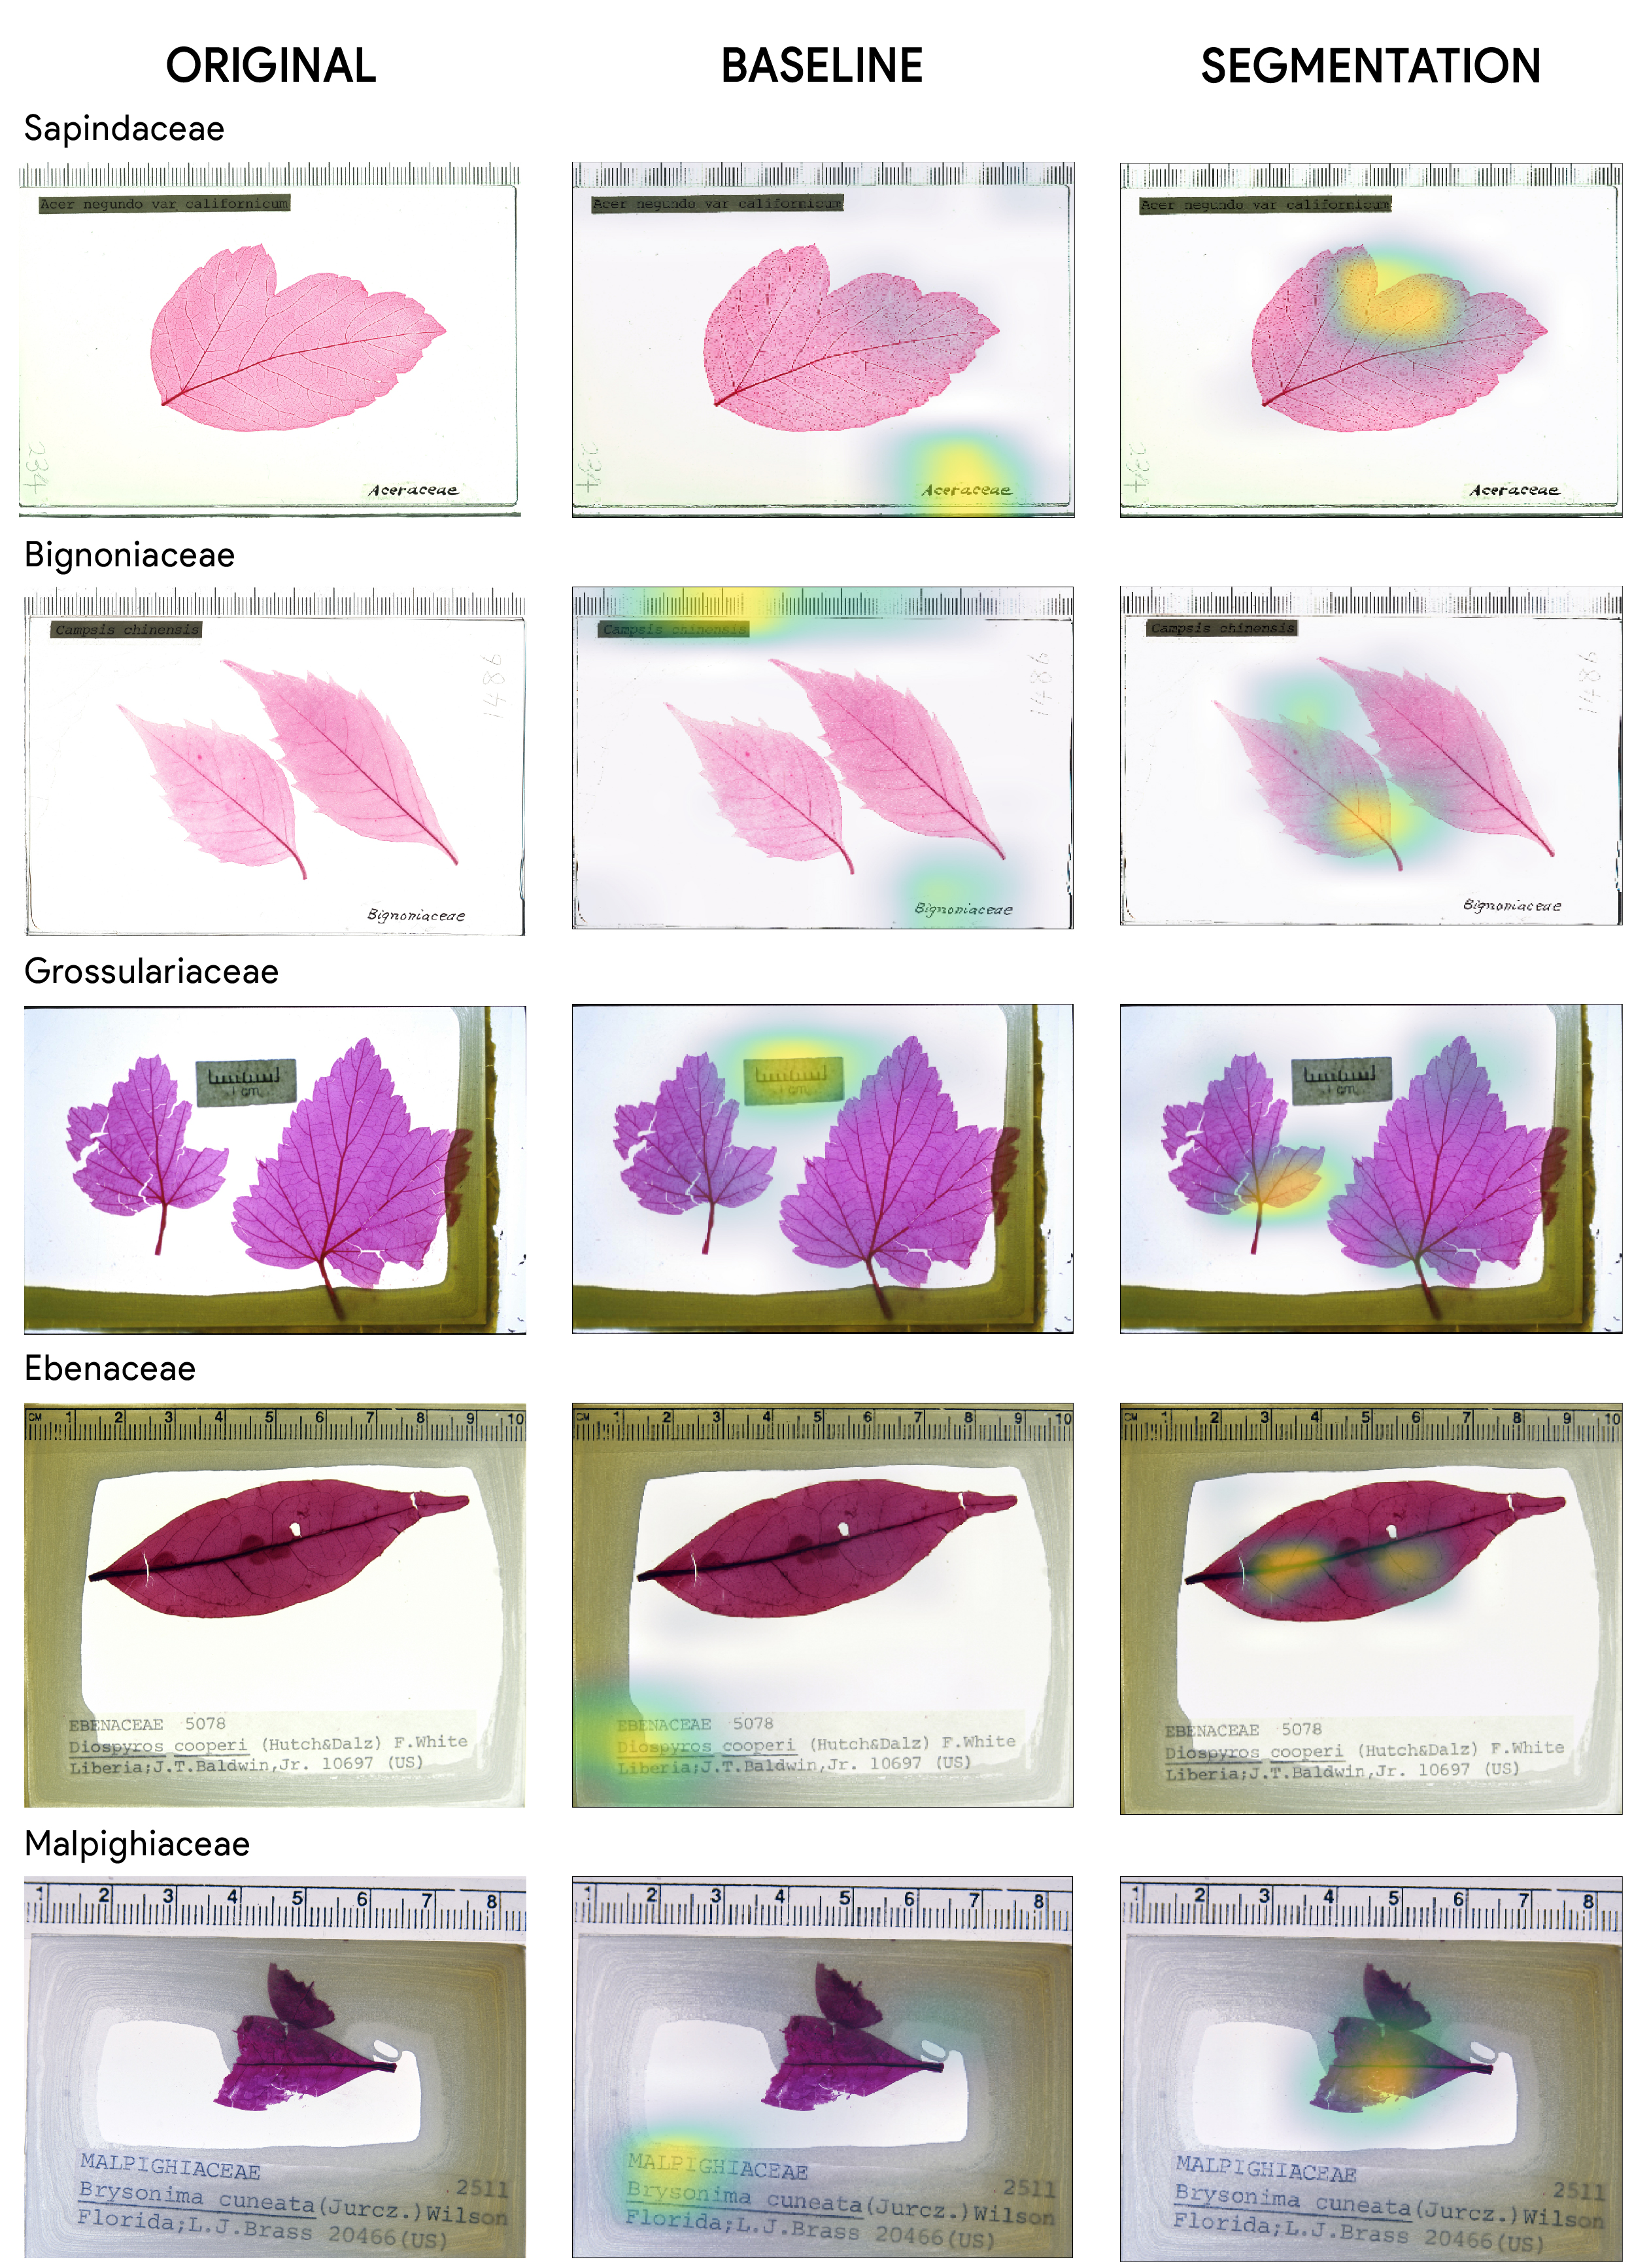
\includegraphics[width=0.6\linewidth]{Figures/SI_Gradcam.jpg}
    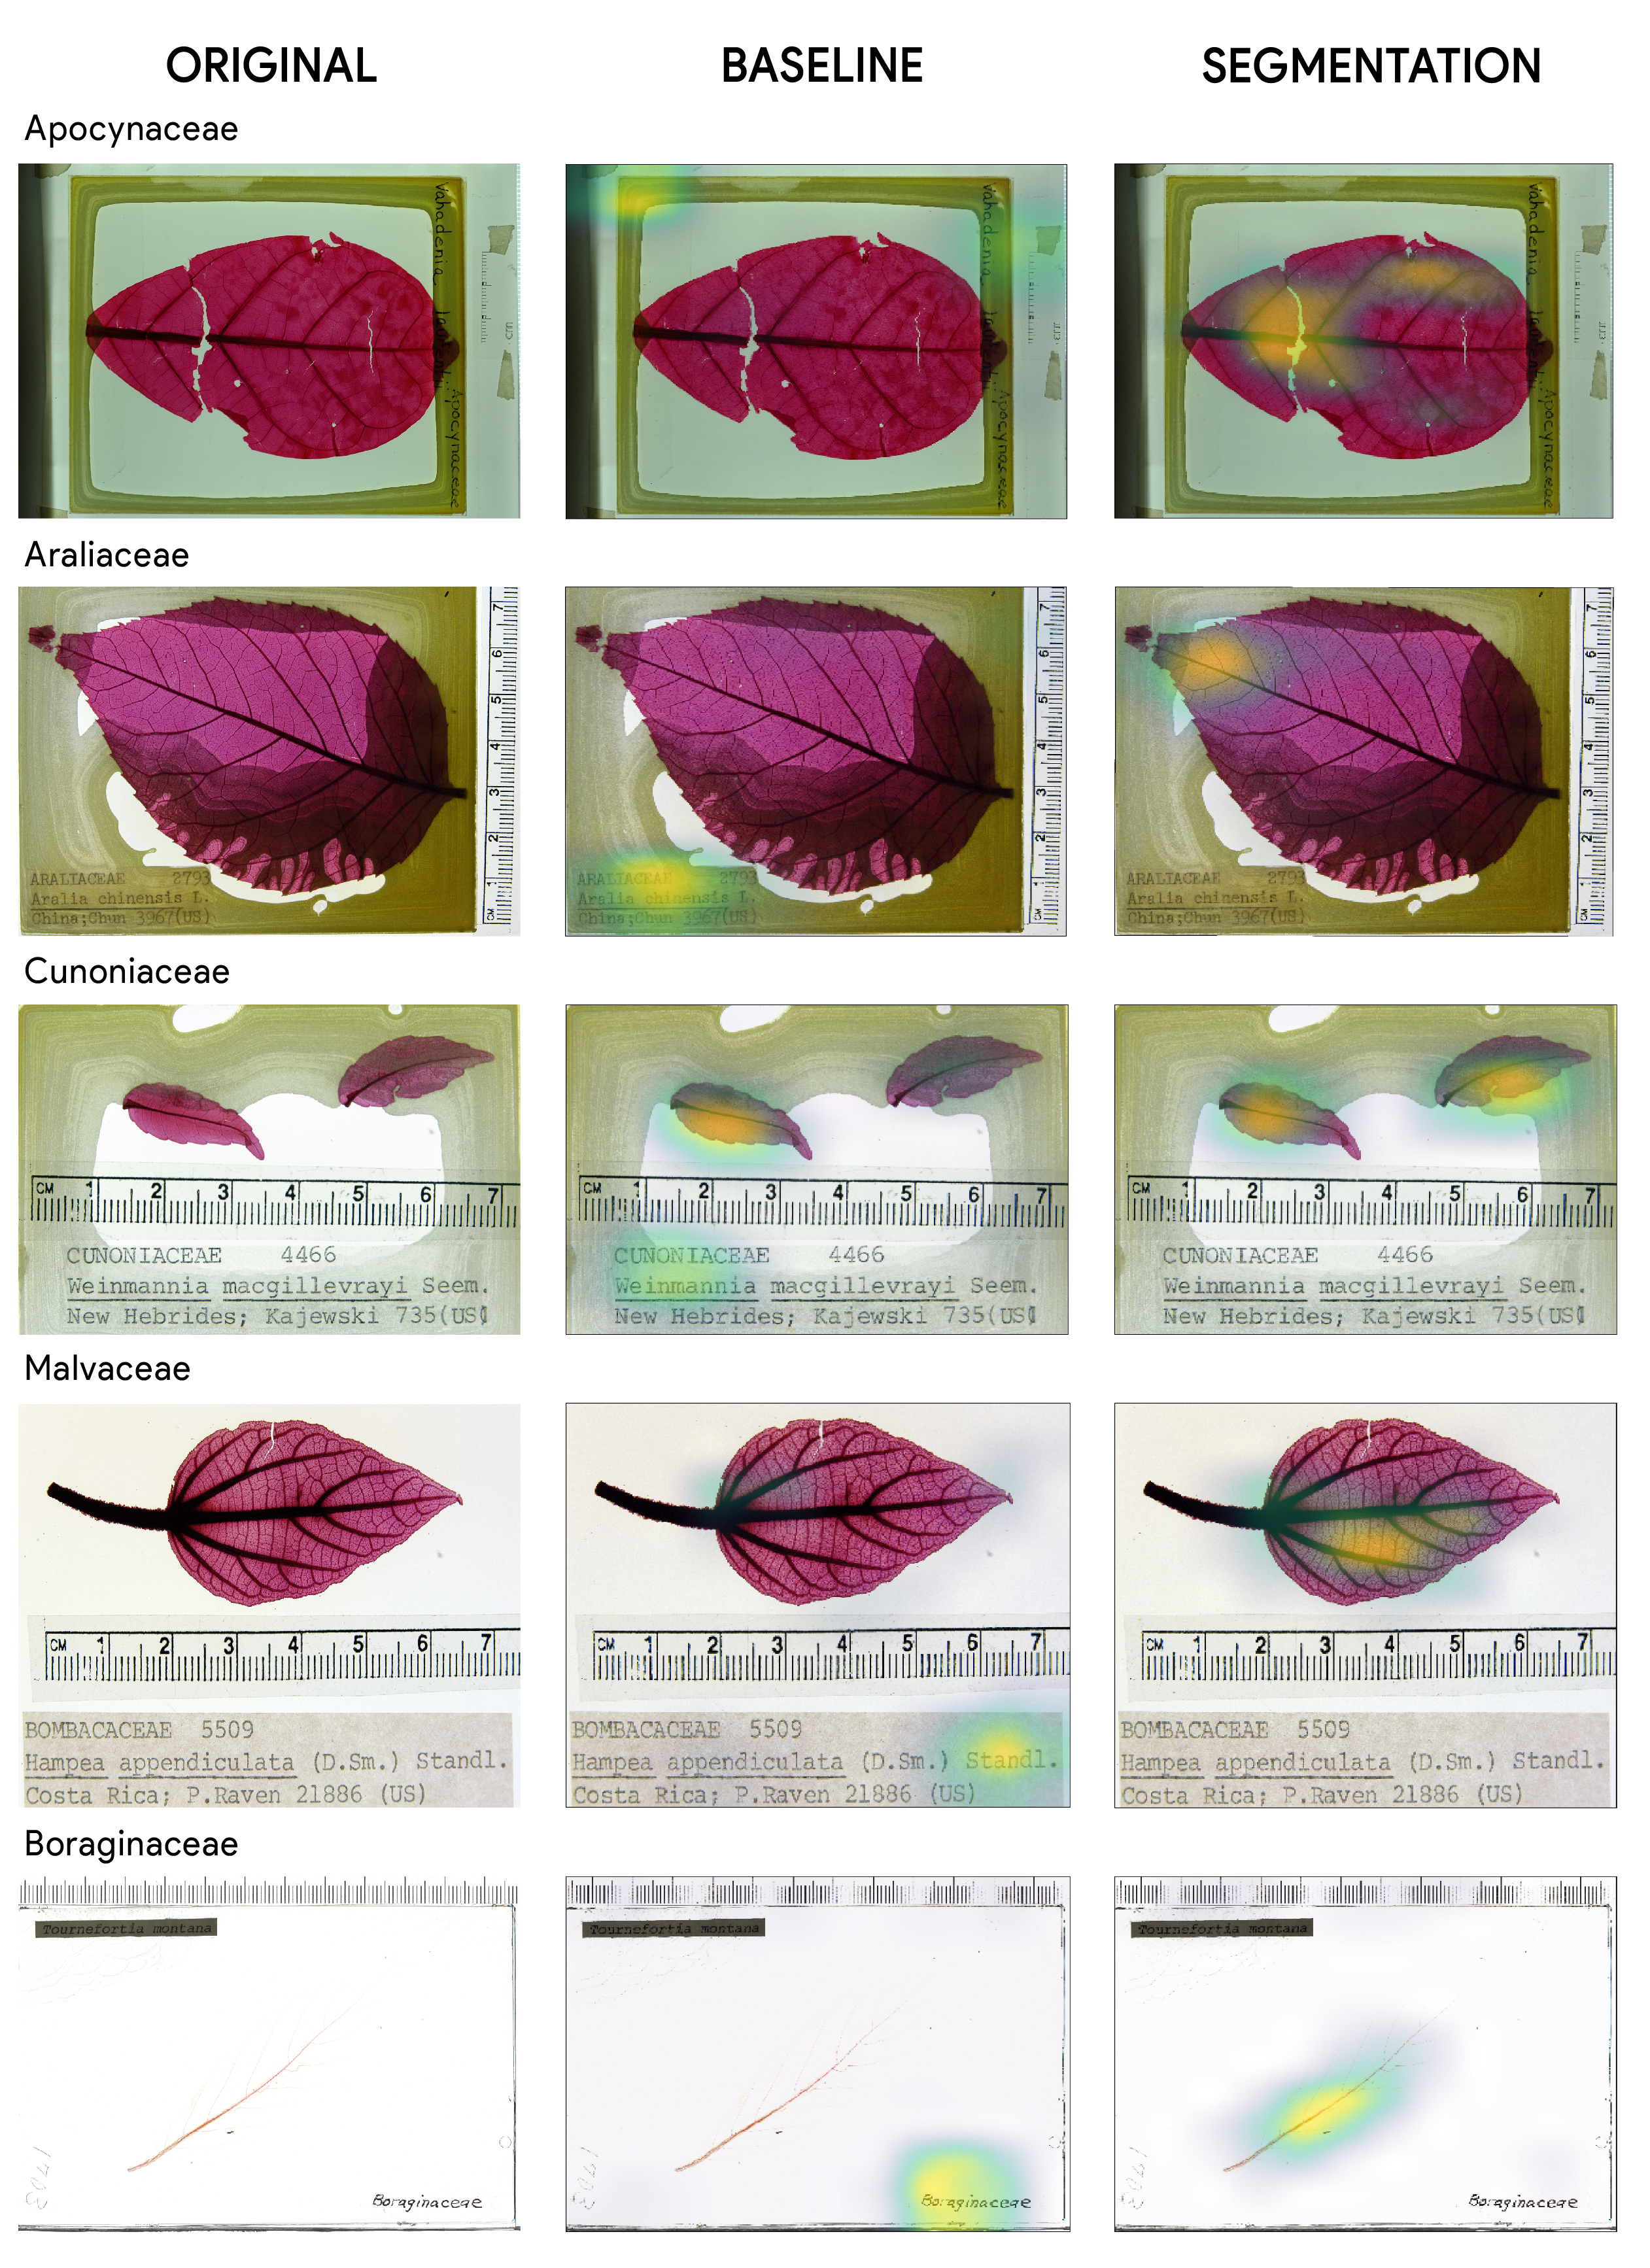
\includegraphics[width=0.6\linewidth]{SI_Gradcam2.jpg}
    \caption{Attribution map generated using Grad-Cam showing before and after segmentation. For each sample , you will find on the left, attributions when no segmentation is performed, showing that the model relies on non leaf features to classify. On the right you will find same sample , but attribution maps from the model trained on segmented leafs.}\label{fig:attribution_maps}
\end{figure}

\clearpage
\subsection{System}
Illustration of the system modules. 
\begin{figure}[ht!]
    \centering
    \includegraphics[width=\linewidth]{Figures/Figure_5_v2.jpg}
     \caption{Illustration of the System. On the left top a represenation of the Leaves domain dataset, we have 142 families. We use them as input of the Controlnet to create synthetic fossils. On the bottom we see a representation of the Fossil dataset, we only have 16 families, but we complete the rest of 142 by using this generative approach. In the middle find the details for the cllasification architecture and the ControlNet prompting approach. Finally, on the right, find the sampling procedure for the triplet calculation, cross-domain and same-domain, taking the furthest positive to bring closer to the anchor and the closest negative to push from the anchor. Finally, right bottom, there is the cycle consistent approach illustration, we take a sample, use controlnet to create a synthetic fossil, then from that fossil we create a synthetic leave that aims fo be as close as possible to the original sample. }
\label{fig:SI_Full_system}
\end{figure}
% \begin{figure}[ht!]

%     \centering
%     \includegraphics[width=\linewidth]{Figures/GradCAM2.png}
%     \caption{Attribution map generated using GradCAM showing before and after segmentation. For each sample , you will find on the left, attributions when no segmentation is performed, showing that the model relies on non leaf features to classify. On the right you will find same sample , but attribution maps from the model trained on segmented leafs. }
%     \label{fig:attribution_maps}
% \end{figure}

\clearpage
\subsection*{Results of BeIT}
We also studied BeIT architecture, however the result shows slightly lower performance than the Resnet101 presented in the main thex. See  Table~\ref{tab:beit} summarizes the Top-5 accuracy For these results :
\begin{table}[ht!]
\centering
{%
\begin{tabular}{|c|c|c|c|}
\hline
Condition &
  \begin{tabular}[c]{@{}c@{}}Top 5\\ Lower Bound\end{tabular} &
  \begin{tabular}[c]{@{}c@{}}Top 5 \\ Upper Bound\end{tabular} &
  \#families \\ \hline
Unsegmented                                                   & 4.21\% & 64.3\% & 142 \\ \hline
Segmented                                                     & 6.21\% & 65.1\% & 142 \\ \hline
\begin{tabular}[c]{@{}c@{}}Triplet +\\ Segmented\end{tabular} & 21.4\% & 72\%   & 142 \\ \hline
\begin{tabular}[c]{@{}c@{}}Triplet + \\ Segmented +\\ Synthetic Fossils\end{tabular} &
  \textbf{75.1\%} &
  \textbf{86.4\%} &
  142 \\ \hline

\end{tabular}%
\caption{BEiT classification results under the different conditions studied.}
}
\label{tab:beit}
\end{table}

\subsection{Details for Training the cycle-control-Net}
We use a Large Memory IBM Node with 4 V100 GPUS and 1tB of RAM with fast interconnect between RAM and GPU. One GPU was exclusively hosting the SAM model trained for image silhouette detection, while the other three hosted the Control Net running on stable difussion 2.1.  The Batch size was 64 with a total resolution of 512x512. 

\subsection*{Additional Concepts}
Find Examples of more concepts that our model finds below, and please Please visit our website \footnote{\url{https://fel-thomas.github.io/Leaf-Lens/}} for an exhaustive list of concepts.  
\begin{figure}
    \centering
    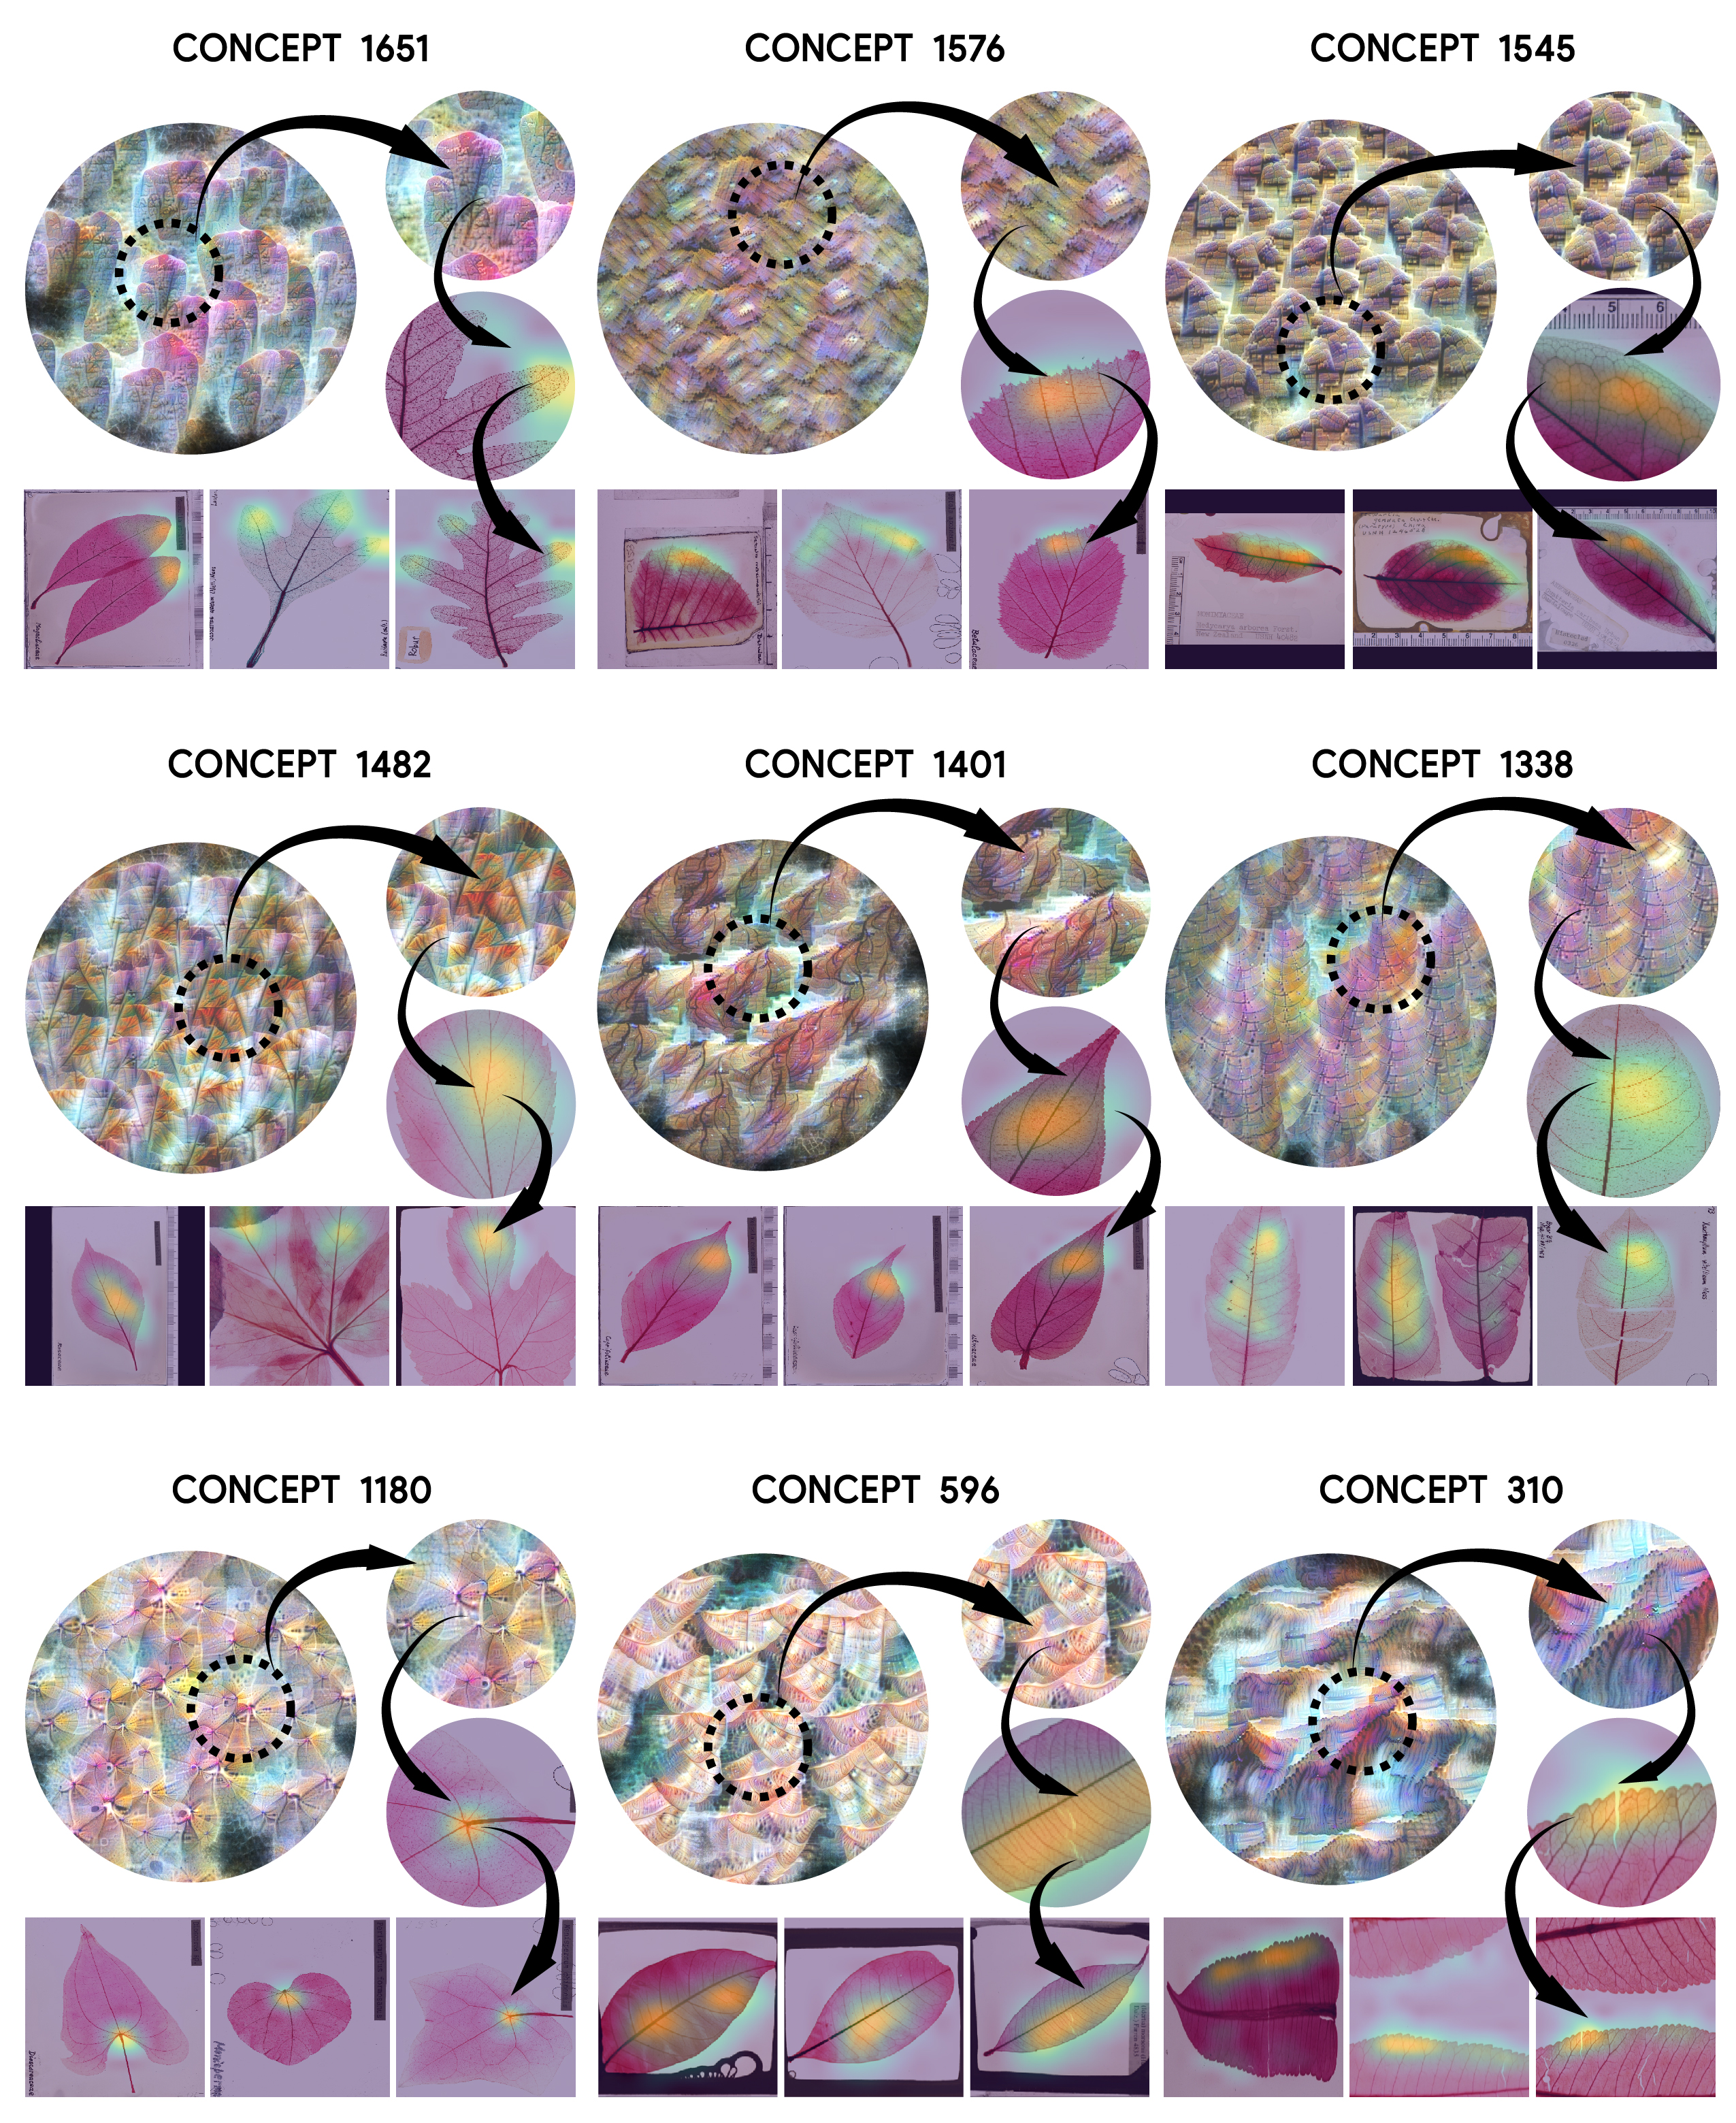
\includegraphics[width=\linewidth]{Figures/SI_6A.jpg}
    
    \caption{Examples of more concepts used by the model. }
    % Footnote moved outside caption

\label{fig:SI_concepts}
\end{figure}


\begin{figure}
    \centering
    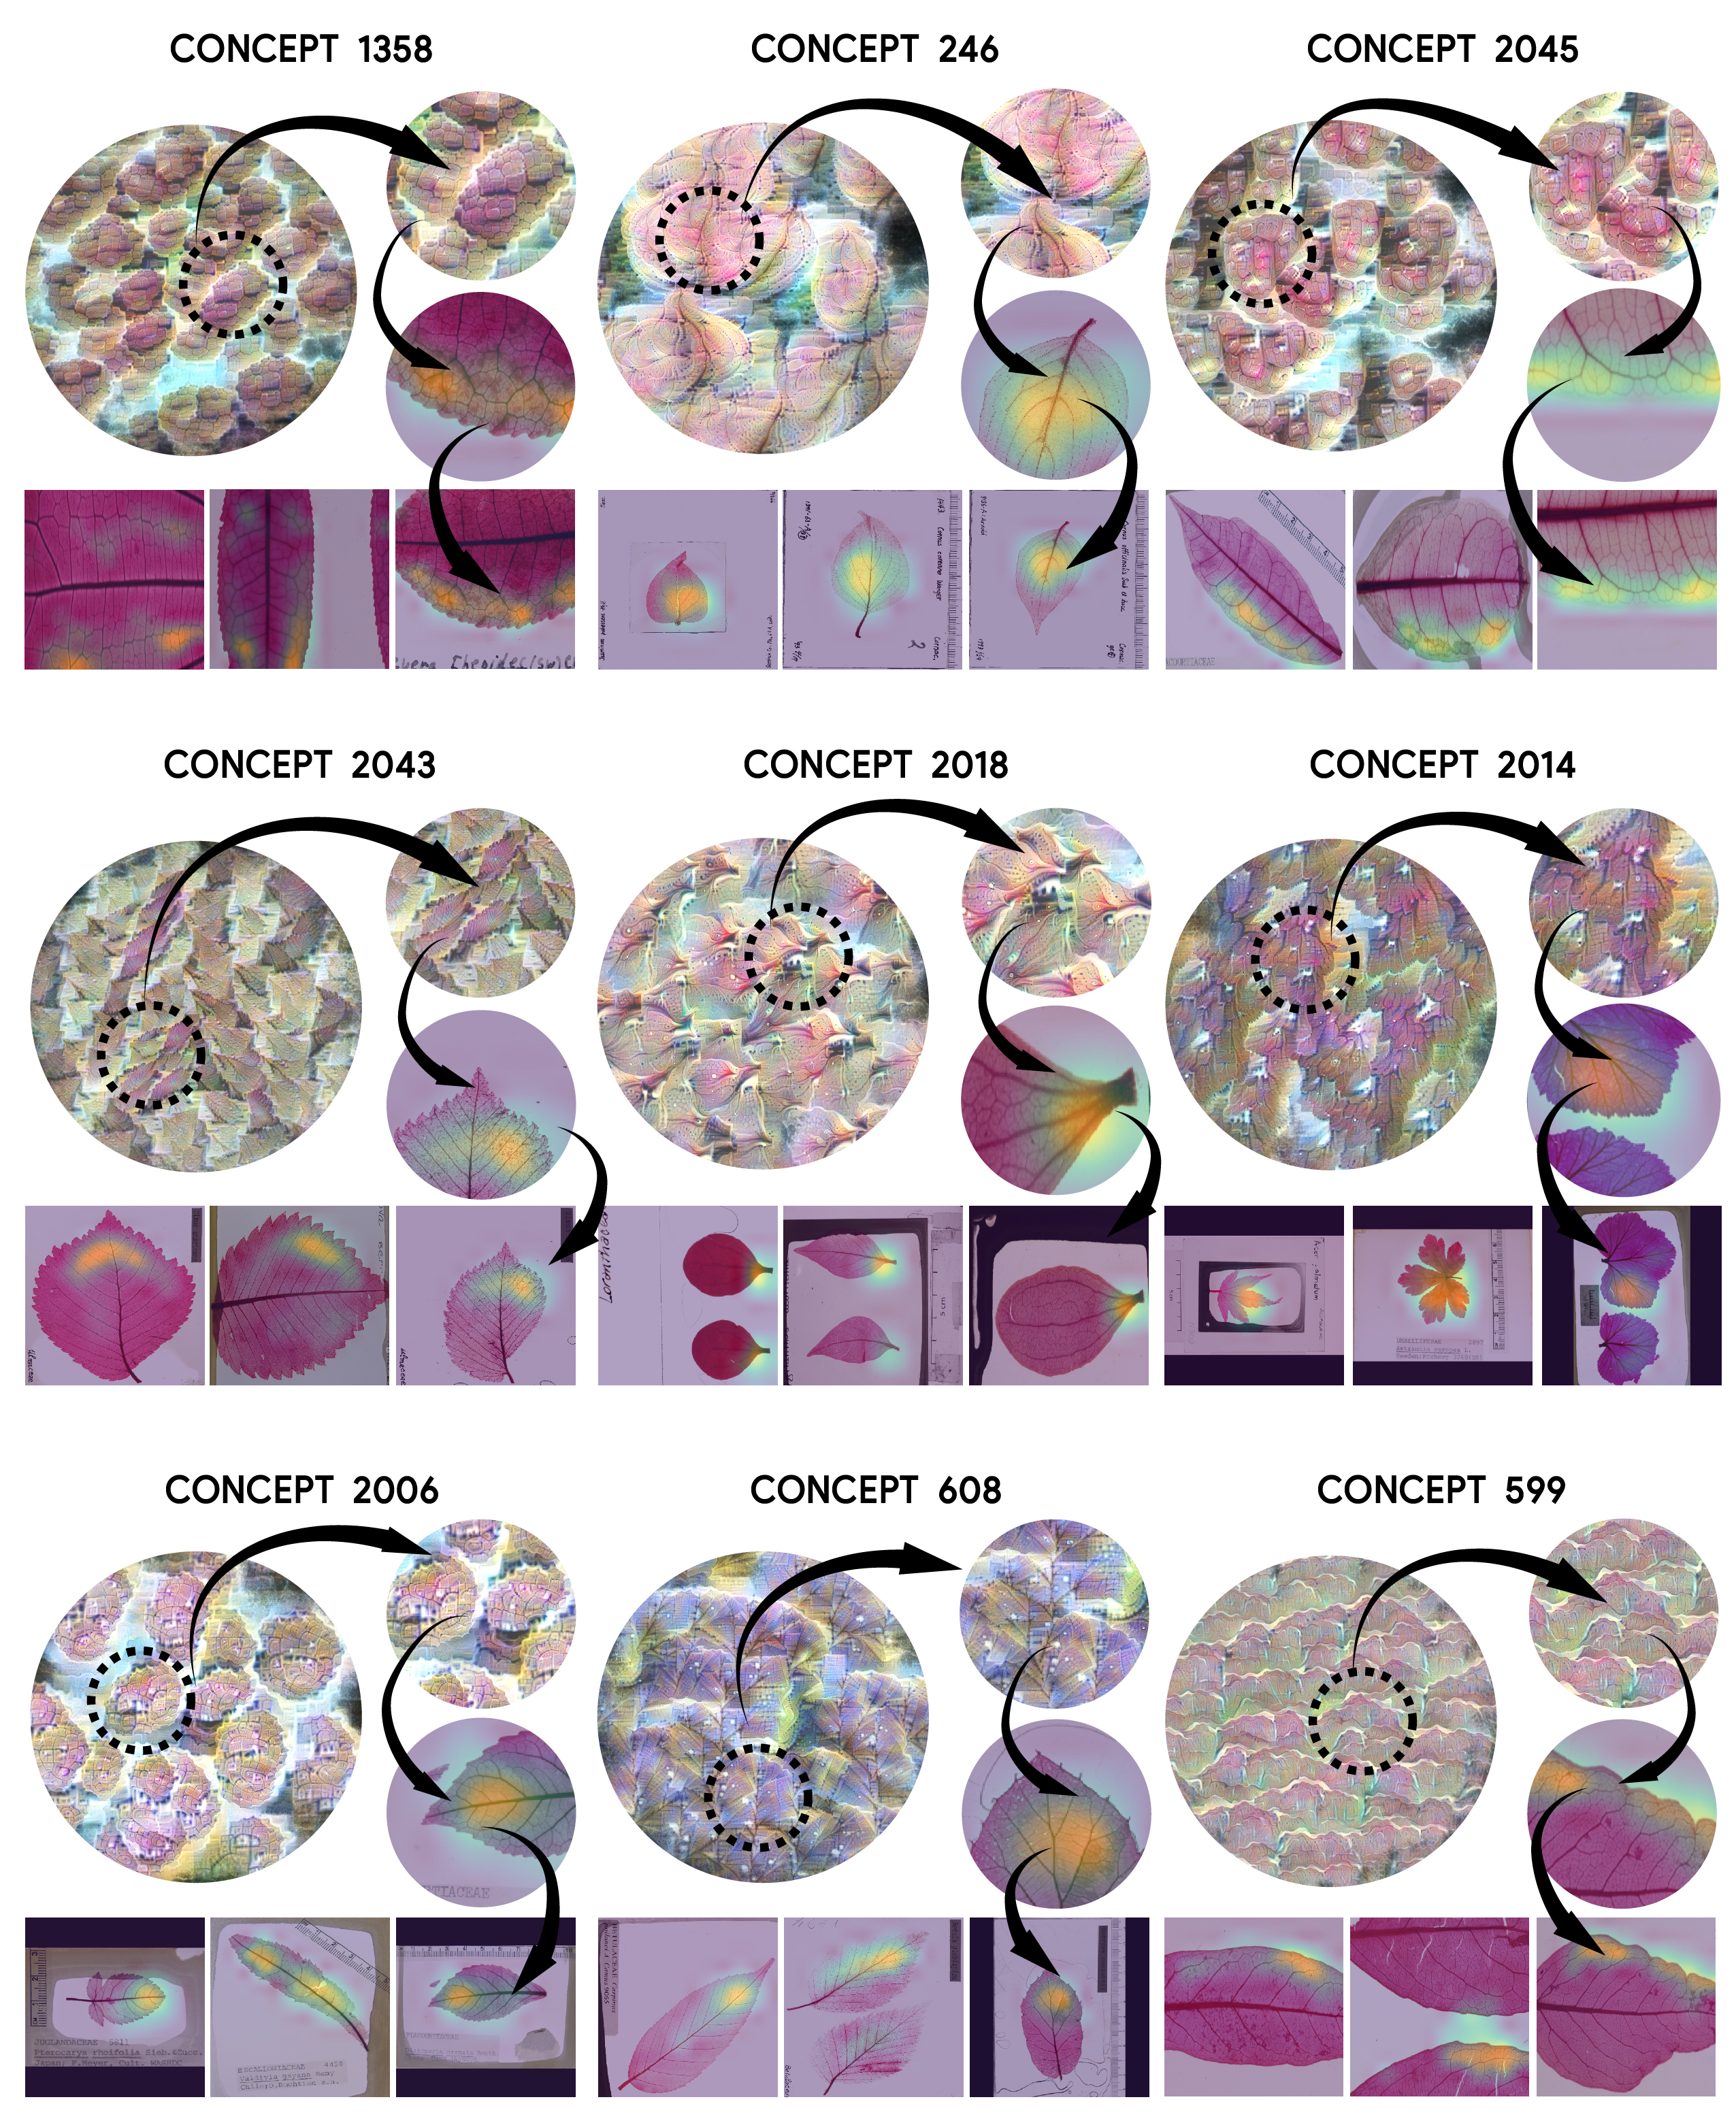
\includegraphics[width=\linewidth]{Figures/SI_6B.jpg}
    
    \caption{Additional examples  of concepts used by the model.}
    % Footnote moved outside caption

\label{fig:SI_concepts2}
\end{figure}

% \bibliographystyle{sn-mathphys}
% \bibliography{sn-bibliography}% common bib file

%% if required, the content of .bbl file can be included here once bbl is generated
%%\input sn-article.bbl

\end{oldappendices}
\end{document}